% !TEX root=../../main_file.tex
% !TeX TS-program = pdflatex
% !TeX checkspelling = fr_toutesvariantes


\chapter{Matériaux et méthodes expérimentales}\label{chap:methods} 
%\chaptermark{Mat. et méth. électrochimiques}
\begin{refsection}
\minitoc

\section{Introduction}
Les principales caractéristiques des matériaux, sélectionnés pour l'étude du phénomène de Shadow Corrosion, 
sont décrites dans un premier temps. 
Dans un second temps, les conditions d'oxydation
en micro-autoclave sont détaillées avec au préalable une description de la manière dont a été simulé l'environnement REB en
termes de température, pression et chimie. Les limitations liées à l'utilisation des micro-autoclaves sont
également abordées.
Enfin, les méthodes électrochimiques classiques utilisées dans ce travail sont présentées avec quelques précisions sur les
difficultés de mesure liées à l'utilisation de cellules électrochimiques métalliques. La technique de mesure en
photoélectrochimie sera abordée au chapitre \ref{chap:design}.

%%%%%%%%%%%%%%%%%%%%%%%%%%%%%%%%%%%%%%%%%%%%%%%%%%%%
\section{Matériaux étudiés}\label{sec:ch2_materials}

    Le chapitre \ref{chap:ch1_bib} a montré que le principal alliage utilisé pour les gaines de confinement est l'alliage
    \emph{Zircaloy-2} alors que le principal alliage utilisé pour les grilles de maintien est l'alliage \emph{Inconel 718}. 
    L'ensemble de nos travaux expérimentaux a été réalisé avec ces alliages
    fournis par Cezus pour le \emph{Zircaloy-2} et Goodfellow pour l'\emph{Inconel 718}, respectivement. Dans la suite, ces deux
    alliages sont dénommés \emph{Zy2} et \emph{Inc718}.   
    
    Les deux alliages sont fournis sous forme de tôle industrielle ayant une épaisseur de \SI{2.96}{\milli\meter} et de
    \SI{1}{\milli\meter} pour Zy2 et Inc718, respectivement. Les compositions chimiques nominales de ces deux
    alliages sont données dans les tableaux \ref{tab:ch2_Zy2_composition} et \ref{tab:ch2_718_composition}. 

    \begin{table}[H]
    \centering
        \begin{tabular}{p{0.08\textwidth}%
                        p{0.081\textwidth}%
                        p{0.08\textwidth}%
                        p{0.08\textwidth}%
                        p{0.08\textwidth}%
                        p{0.08\textwidth}%
                        p{0.08\textwidth}%
                        p{0.09\textwidth}%
                        p{0.09\textwidth}}
            \toprule
            \textbf{Ref. \newline Cezus} & Zr & Sn & Fe & Cr & Ni & O (ppm) & Si (ppm) & C (ppm) \\\midrule
            810393 & Bal. & 1.32 & 0.169 & 0.108 & 0.055 & 1170 & 107 & 157 \\
            \bottomrule
        \end{tabular}

    \caption[Composition chimique de l'alliage Zy2.]
    {Composition chimique de l'alliage Zy2 exprimée en pourcentage massique sauf indication contraire.}
    \label{tab:ch2_Zy2_composition}
    \end{table}


    \begin{table}[H]
    \centering
        \begin{tabular}{p{0.2\textwidth}%
                        p{0.1\textwidth}%
                        p{0.1\textwidth}%
                        p{0.1\textwidth}%
                        p{0.1\textwidth}%
                        p{0.1\textwidth}%
                        p{0.1\textwidth}}
            \toprule
            \textbf{Ref. \newline Goodfellow} & Ni & Cr & Fe & Nb & Mo & Ti \\\midrule
            LS412242MKS & 53 & 19 & 19 & 5 &3 & 1 \\
            \bottomrule
        \end{tabular}

    \caption[Composition chimique de l'alliage Inc718.]
    {Composition chimique de l'alliage Inc718 exprimée en pourcentage massique.}
    \label{tab:ch2_718_composition}
    \end{table}

    Les
    différents échantillons de l'étude ont été prélevés sur ces tôles industrielles par une découpe fil. 
    L'état de surface initial des échantillons a consisté en un polissage au papier abrasif de grade P1200.

    La figure \ref{subfig:ch2_Zy2_microstructure_optical} montre la microstructure de l'alliage Zy2 observée au
    microscope optique en lumière polarisée. La taille de grain est d'environ une dizaine de microns. Les précipités
    sont distribués de manière homogène aux joints de grains et dans les grains comme on peut le constater sur le cliché MET de la
    figure \ref{subfig:ch2_Zy2_SPPs_MET}. La taille moyenne des précipités est de \SI{150}{\nano\meter}.

     Les échantillons Inc718 ont été traités thermiquement sous air afin de simuler le procédé de conditionnement des
    grilles de maintien avant leur mise en réacteur. Le traitement thermique effectué est schématisé en figure
    \ref{fig:ch2_thermal_treat}.
    L'oxyde formé lors du traitement thermique est ensuite éliminé par polissage au papier
    abrasif de grade P1200.

    \begin{figure}[H]
    \centering
        \begin{subfigure}[b]{0.5\textwidth}
            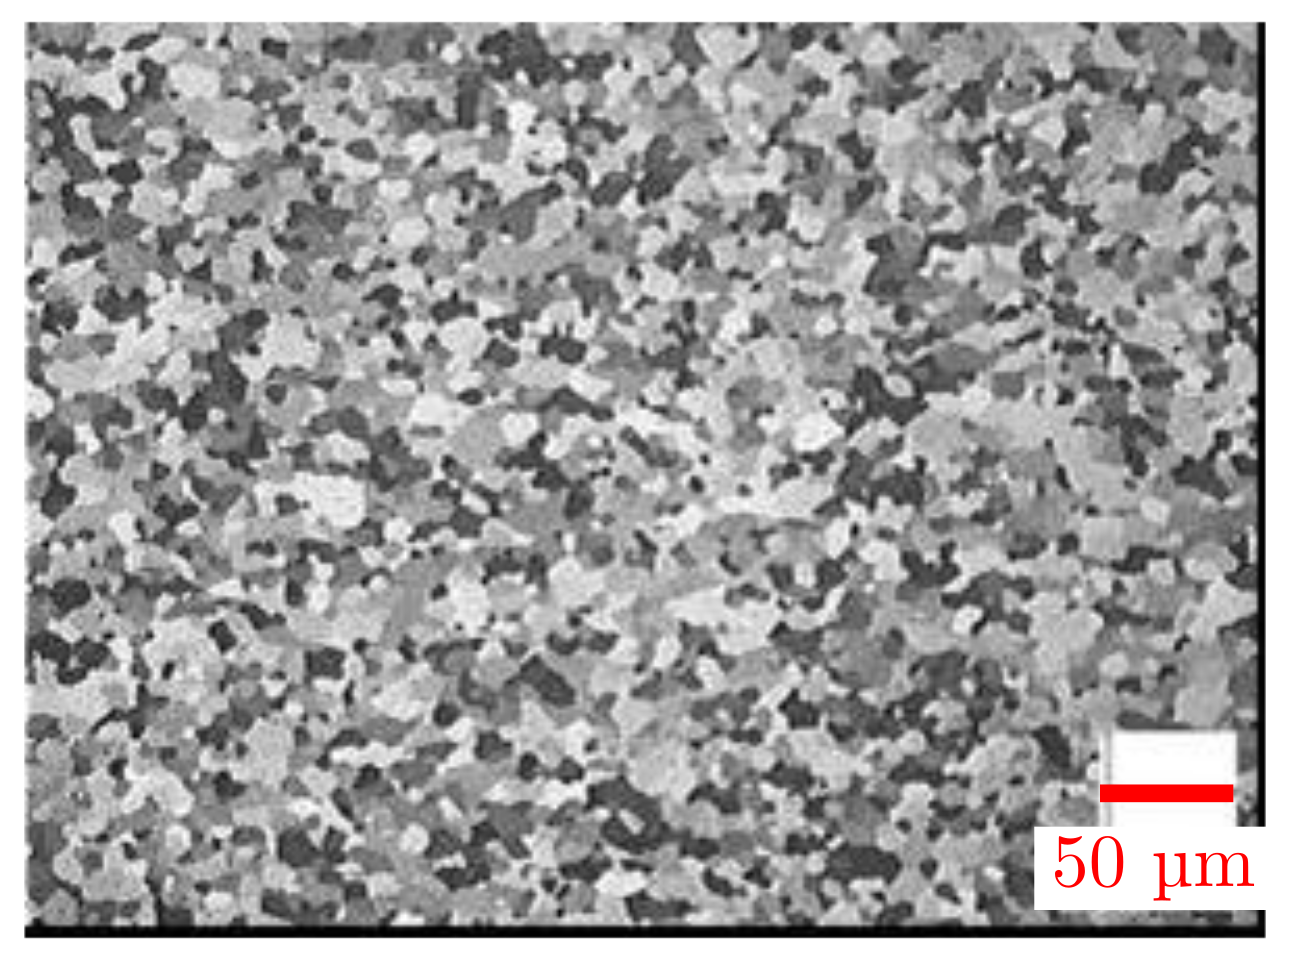
\includegraphics[width=\textwidth]{Guerin_2007-Fig2-redraw.png} 
			\caption{}
			\label{subfig:ch2_Zy2_microstructure_optical}
        \end{subfigure}
        \quad
        \begin{subfigure}[b]{0.4\textwidth}
            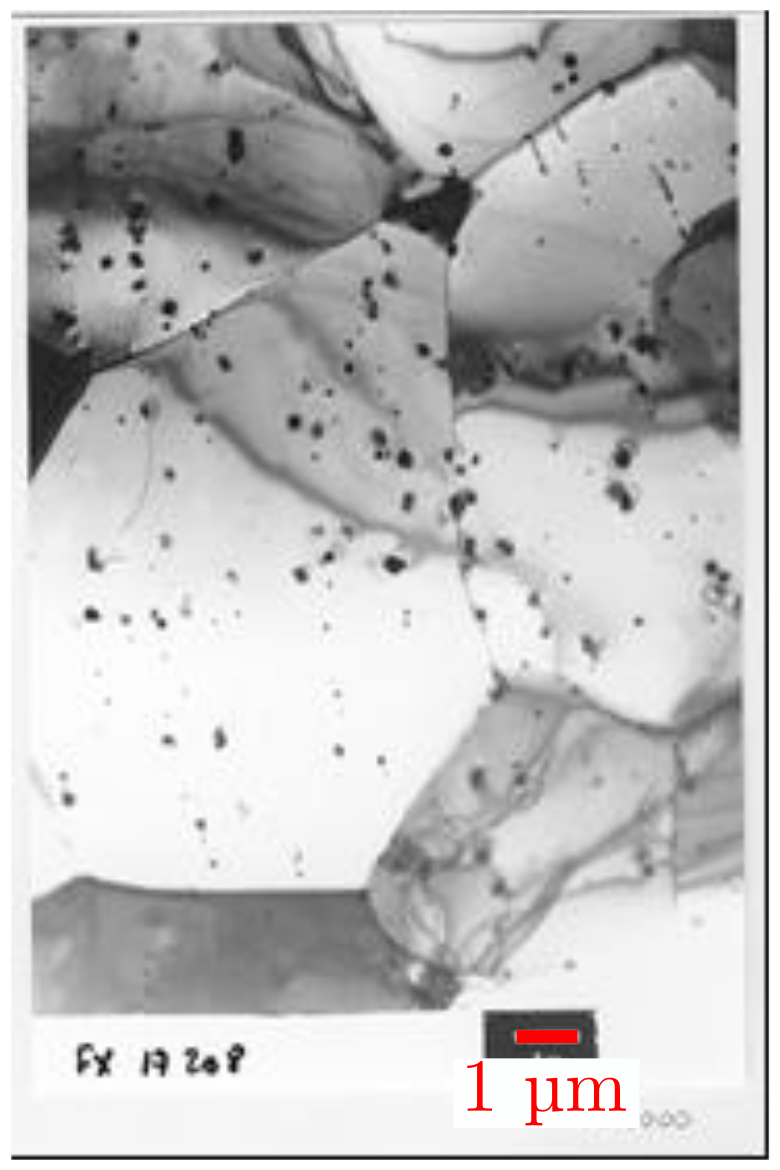
\includegraphics[width=\textwidth]{Guerin_2007-Fig10-redraw.png} 
			\caption{}
			\label{subfig:ch2_Zy2_SPPs_MET}
        \end{subfigure}
    \caption[Microstructure de l'alliage Zy2]
    {Microstructure de l'alliage Zy2: 
            a) cliché optique en lumière polarisée (X200),
            b) cliché MET \citep{Guerin2007}.}
    \label{fig:ch2_microstructure}
    \end{figure}    

    \begin{figure}[H]
        \centering
            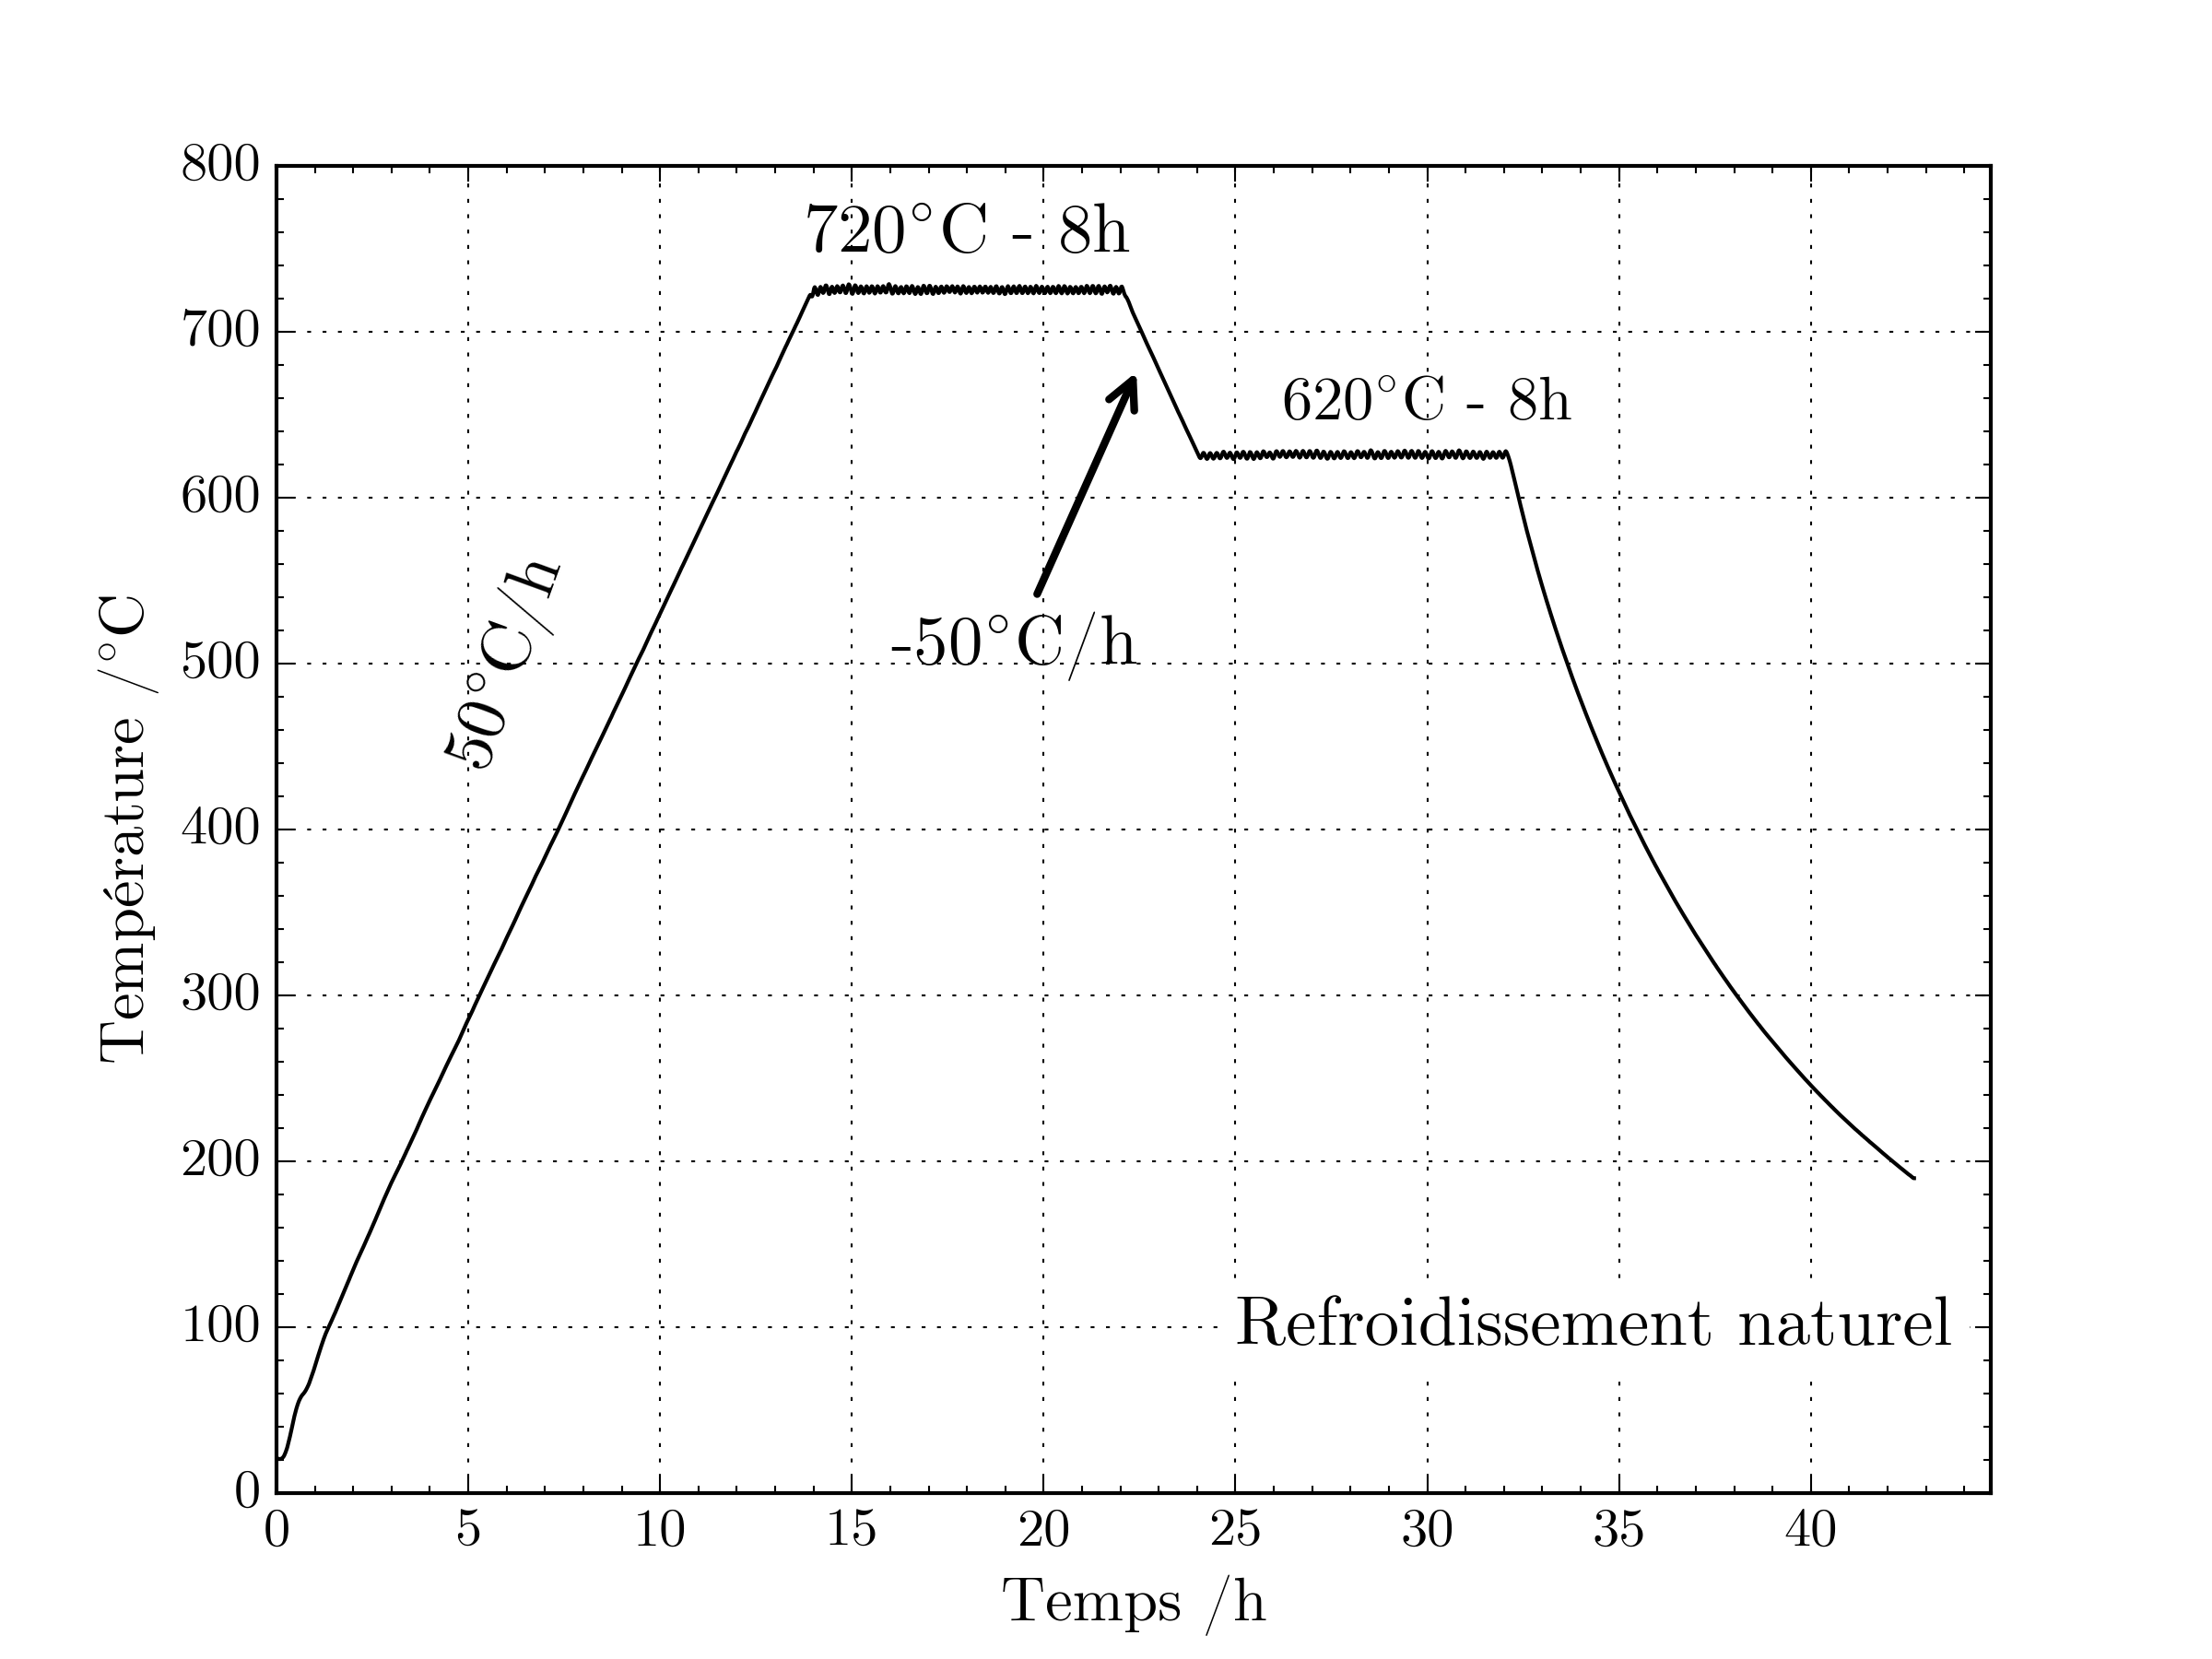
\includegraphics[width=0.65\textwidth]{140778-ATT-X718.png}
        \caption{Traitement thermique appliqué aux échantillon de Inc718 pour simuler le procédé de conditionnement
        des grilles de maintien avant leur mise en réacteur.}
        \label{fig:ch2_thermal_treat}
    \end{figure}

    Trois géométries d'échantillons ont été utilisées, \emph{coupon rectangulaire}, \emph{disque} et \emph{anneau}, 
    dont les représentations schématiques sont
    fournies en figure \ref{fig:ch2_samples_schemes}. Les coupons rectangulaires ont
    seulement été utilisés en micro-autoclaves. En effet, cette géométrie est adaptée à la géométrie longiligne des
    micro-autoclave (\S\ref{sec:ch2_MA_oxydation}) et facilite la prise de contact pour les mesures
    électrochimiques (\S\ref{sec:ch2_electrochemistry}) grâce à la queue de contact en extrémité. 
    Les géométries disque et anneau ont été utilisées dans la cellule électrochimique haute température développée dans le cadre du présent travail
    de thèse. Le détail lié au choix de ces géométries seront abordés au chapitre \ref{chap:design}.

%    \begin{figure}[!htb]
%    \centering
%        \begin{subfigure}[b]{0.75\textwidth}
%            
\includegraphics[width=\textwidth]{140778-Sample_Size-Coupons.png} 
%			\caption{}
%			\label{subfig:ch2_coupons_scheme}
%        \end{subfigure}
%        \quad
%        \begin{subfigure}[b]{0.15\textwidth}
%            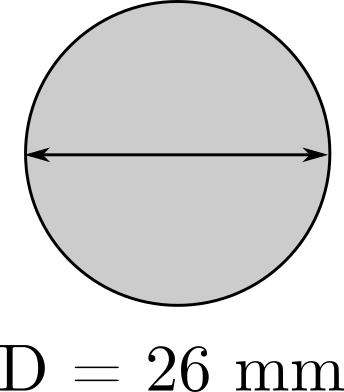
\includegraphics[width=\textwidth]{140778-Sample_Size-Disc.png} 
%			\caption{}
%			\label{subfig:ch2_disc_scheme}
%        \end{subfigure}
%    \caption{Représentation schématique de la géométrie des échantillons: a) coupon, b) disque.}
%    \label{fig:ch2_samples_schemes}
%    \end{figure} 

    \begin{figure}[H]
        \centering
        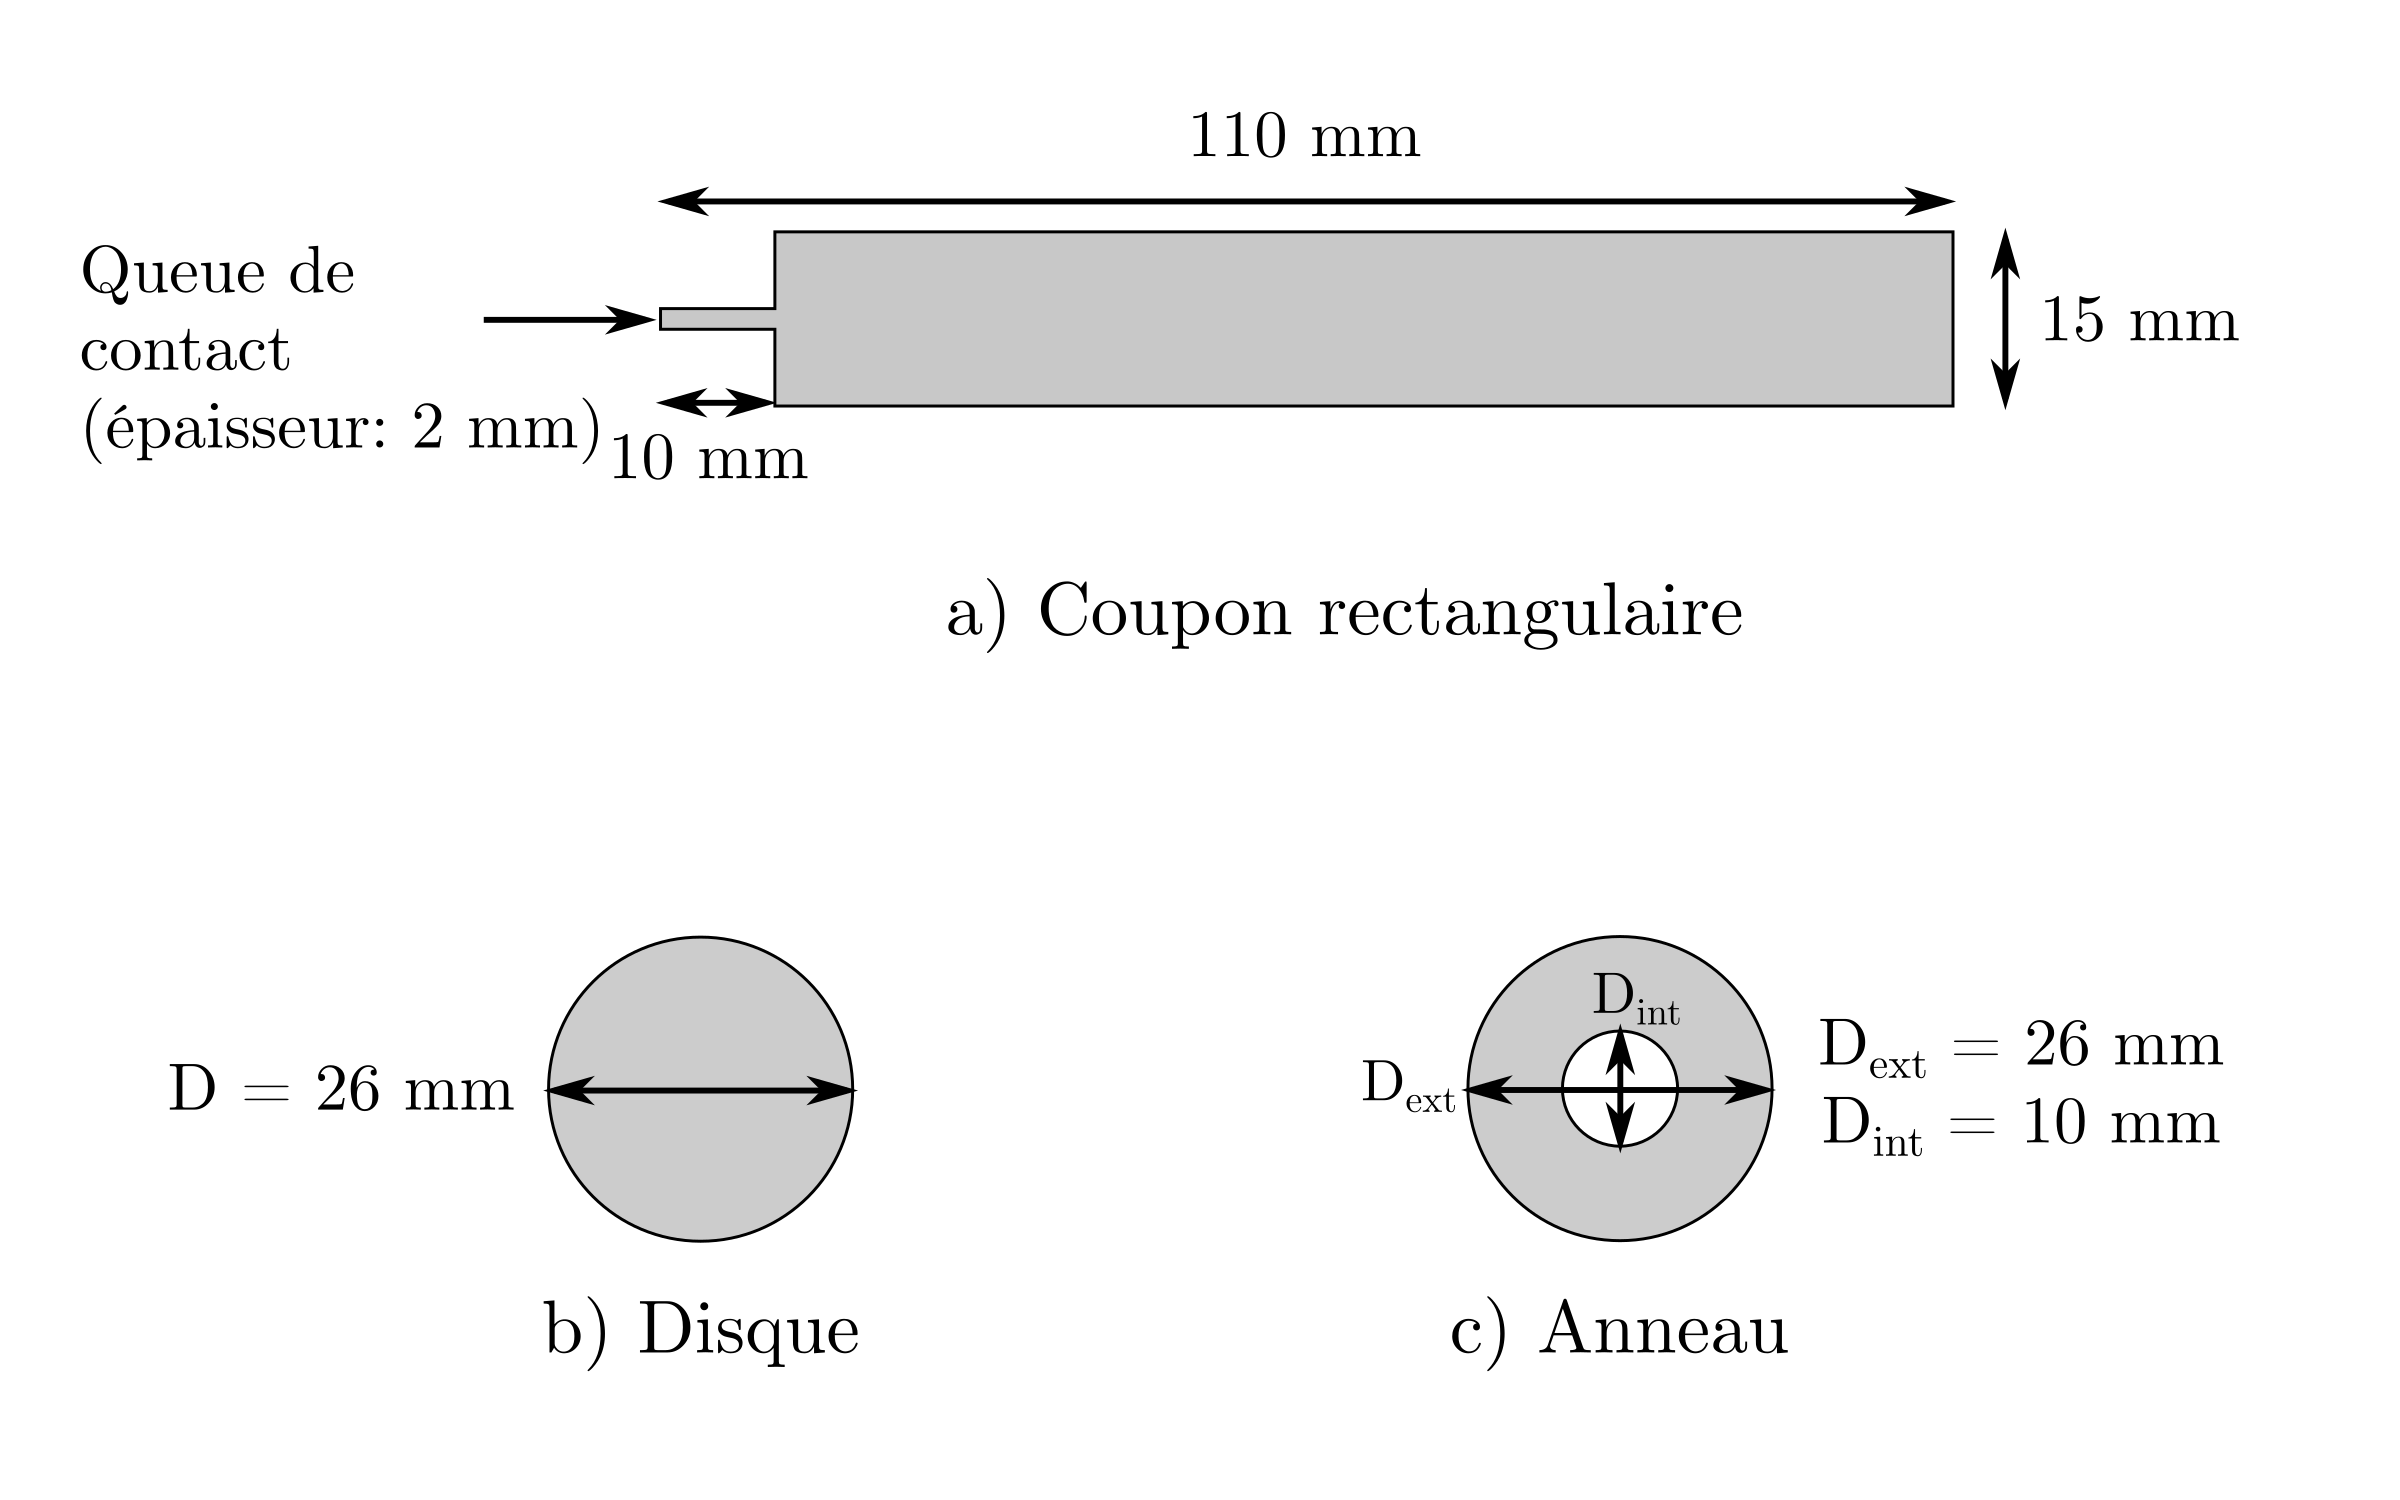
\includegraphics[width=0.85\textwidth]{140778-Sample_Only.png}
        \caption{Représentation schématique de la géométrie des échantillons: a) coupon rectangulaire, b) disque, c)
        anneau.}
        \label{fig:ch2_samples_schemes}
    \end{figure}


%%%%%%%%%%%%%%%%%%%%%%%%%%%%%%%%%%%%%%%%%%%%%%%%%%%
\section{Simulation de l'environnement REB}\label{sec:ch2_T_P}

    Le tableau \ref{tab:operating_parameters_reactors} du chapitre \ref{chap:ch1_bib} montre que la température d'un
    réacteur à eau bouillante varie entre 272 et \SI{278}{\degreeCelsius} à l'entrée et entre 280 et
    \SI{300}{\degreeCelsius} à la sortie pour une pression comprise entre 70 et 80~bars. De plus, les réacteurs à
    eau bouillante sont des réacteurs diphasiques avec la présence de vapeur d'eau générée directement au niveau des
    gaines de confinement du combustible. 

    Le contrôle de l'ébullition au niveau des échantillons lors d'essais de corrosion en laboratoire n'est pas simple
    à obtenir. De plus, la présence d'ébullition ne facilite pas les mesures électrochimiques puisque les bulles de
    vapeur masquent une partie de la surface de l'échantillon et rendent difficile la normalisation des courants mesurés par
    rapport à la surface exposée.

    Afin de s'affranchir de ces potentiels problèmes expérimentaux liés à la présence de phase vapeur, il a été décidé de
    travailler en milieu monophasique. Par conséquent, le milieu REB a été simulé en fixant la température à sa valeur
    basse de sortie, soit \SI{280}{\degreeCelsius}, sous une pression de \SI{80}{\bar}.

    L'électrolyte utilisé ici pour simuler le milieu REB est de l'eau ultra-pure 
    dans laquelle on peut faire varier la teneur en oxygène dissous ainsi que la
    concentration en autres composés chimiques. 
    La manière dont la teneur en oxygène dissous a été contrôlée finement sera abordée au chapitre \ref{chap:design}.
    Le
    détail des compositions chimiques des électrolytes utilisées pour nos expériences sera donné au cours de l'exposé
    des résultats au chapitre 4.
    %\ref{chap:ch4_results}.

    Il convient de rappeler ici que l'eau ultra-pure présente une faible conductivité de l'ordre de 
    \SI{0.06}{\micro\siemens\per\centi\meter} à température ambiante et de \SI{3}{\micro\siemens\per\centi\meter} à
    \SI{280}{\degreeCelsius} \citep{IAEA1997}. Cette conductivité limitée aura pour conséquence une chute
    ohmique élevée entre l'échantillon et la référence de potentiel dans la cellule électrochimique haute température. 
    
     
   

%%%%%%%%%%%%%%%%%%%%%%%%%%%%%%%%%%%%%%%%%%%%%%%%%%%%
\section[Oxydation des matériaux en micro-autoclave statique]%
{Oxydation des matériaux en micro-autoclave statique}\label{sec:ch2_MA_oxydation}

    Les micro-autoclaves, en alliage de nickel A600, sont sous forme de tube avec 
    un diamètre interne de \SI{40}{\milli\meter} et une hauteur
    d'environ \SI{230}{\milli\meter}. Ils sont préalablement aux expériences, 
    passivés en eau ultra pure à \SI{280}{\degreeCelsius}
    afin de
    limiter par la suite la pollution de l'électrolyte par relâchement issus du contenant.
    %Par la suite, les cinq micro-autoclaves que nous avons
    %utilisés sont identifiés par \emph{MA1} \ldots \emph{MA5}. 
    Une représentation schématique d'un tel micro-autoclave est
    présentée en figure \ref{fig:ch2_MA_scheme}.

    
    Ces micro-autoclaves sont équipés de passages étanches pour les fils assurant le contact électrique avec
    les coupons rectangulaires. Ils sont maintenus parallèles avec un support en PEEK, fourni par l'usineur
    \emph{Micro2000}, spécifiquement
    conçu pour cette géométrie. La distance entre les deux coupons rectangulaires a été fixée à \SI{10}{\milli\meter}. L'isolation
    électrique entre les différents fils de contact est assurée par des gaines thermo-rétractables en PTFE fourni par
    \emph{REA}. Le contact
    entre les fils et la queue des coupons rectangulaires est assuré par une bague équipée d'une vis de serrage. La nature des
    matériaux des fils et des bagues est identique à celle des coupons rectangulaires pour lesquels ils assurent le contact électrique.
   
    Le volume d'électrolyte à injecter a été calculé en tenant compte du changement de masse volumique de l'eau à
    \SI{280}{\degreeCelsius}. La hauteur d'immersion visée pour les coupons rectangulaires
    était d'environ \SI{90}{\milli\meter}, a été systématiquement vérifiée après exposition. Cette hauteur
    d'immersion permet de garder les points de contact électrique dans un ciel d'argon. La pression initiale d'argon, avant la mise en
    chauffe, a été fixée à \SI{10}{\bar} permettant d'atteindre environ \SI{80}{\bar} lorsque la température atteint
    \SI{280}{\degreeCelsius}. 
    
    L'homogénéité thermique du four permettant de chauffer les micro-autoclaves n'étant pas
    parfaite, les micro-autoclaves n'étaient pas tous strictement à la même température. Typiquement, le
    micro-autoclave le plus froid est à environ \SI{275}{\degreeCelsius} alors que le plus chaud est à environ \SI{
    285}{\degreeCelsius} lorsque la température visée est de \SI{280}{\degreeCelsius}
       
    Le contrôle fin de la concentration en oxygène dissous en micro-autoclave statique n'est pas possible à obtenir.    
    Par conséquent, les électrolytes ont été systématiquement désaérés pendant \SI{1}{\hour} avant d'être chargés 
    dans les micro-autoclaves, il a été estimé que cette procédure conduisant à une teneur en oxygène dissous de
    moins de \SI{10}{\ppb}. De plus, ce milieu
    désaéré permet d'utiliser le platine comme pseudo-référence de potentiel.

    Des échantillons de géométrie disque et anneau ont également été placés au fond des micro-autoclaves sur des supports
    spécifiques en PEEK, 
    pour servir d'échantillons de référence, c'est-à-dire n'ayant pas été galvaniquement couplé. 
    Les disques ainsi que les anneaux ont par ailleurs une géométrie adaptée à la cellule électrochimique haute
    température, ce qui permettra leur caractérisation (photo-)électrochimique.
    
    \begin{figure}[H]
        \centering
            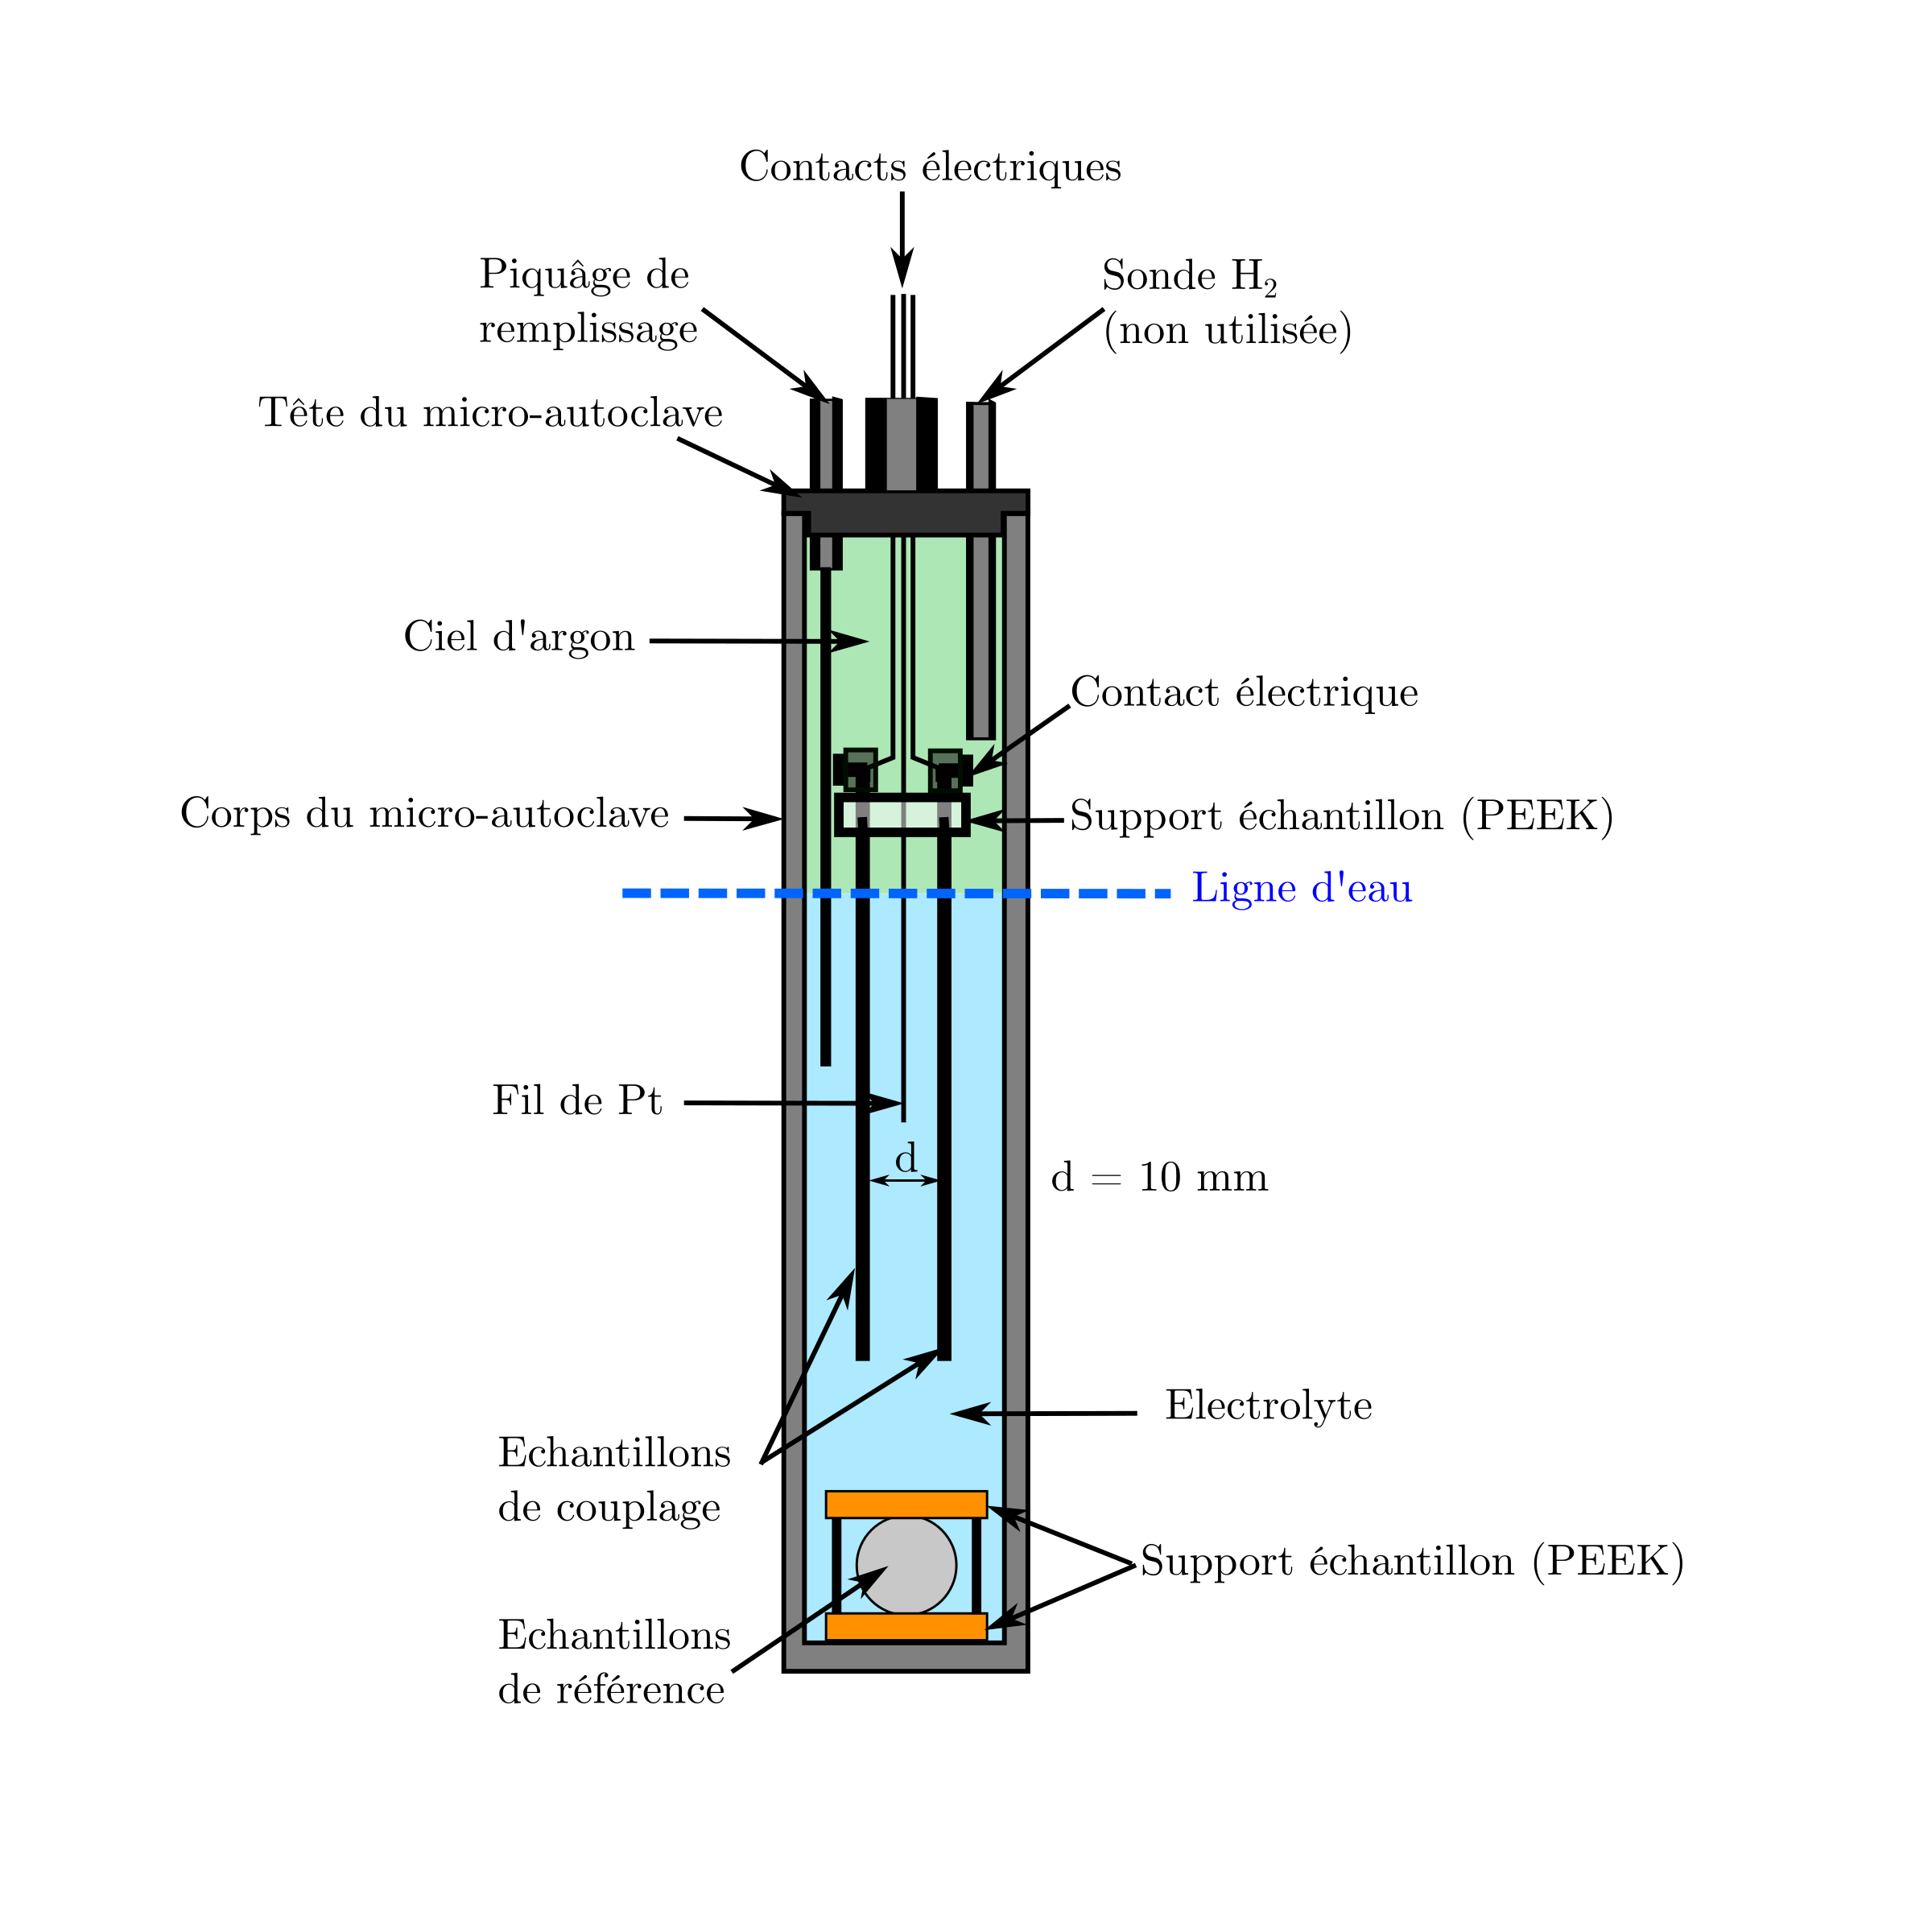
\includegraphics[width=0.95\textwidth]{140778-MA-Setup.png}
        \caption{Représentation schématique du micro-autoclave instrumenté.}
        \label{fig:ch2_MA_scheme}
    \end{figure}
   
    

%%%%%%%%%%%%%%%%%%%%%%%%%%%%%%%%%%%%%%%%%%%%%%%%%%%%
\section{Mesures des prises de masse}\label{sec:ch2_weighting}

    Les variations de masses, $\Delta m$, liées à l'oxydation ont été déterminées par pesée des échantillons avant 
    et après exposition en micro-autoclave
    avec une balance \emph{Sartorius Cubis} ou une balance \emph{Sartorius Secura}, ayant une résolution de
    \SI{0.01}{\milli\gram},
    en suivant le protocole de pesée en vigueur au Centre Technique du Creusot \citep{Perche2015}: les échantillons sont pesés
    trois fois de manière non consécutive. Si l'écart entre la valeur maximale et la valeur
    minimale est inférieureà \SI{0.05}{\milli\gram}, les pesées sont considérées comme valides. 
    
    Les surfaces exposées ont été obtenues en mesurant trois fois les dimensions
    caractéristiques: hauteur, largeur, épaisseur dans le cas des coupons rectangulaires et diamètre,
    épaisseur
    dans le cas des disques et des anneaux. Les mesures sont effectuées avec un pied à coulisse numérique \emph{Mitutoyo
    CD20MAX} ayant une résolution de \SI{0.01}{\milli\meter}.

    Les incertitudes sur les mesures de gains de masse par unité d'aire, $\Delta m /A$, ont été calculées en utilisant la méthode 
    de propagation des erreurs \citep{Protassov2002,Bevington2003}. 
    Pour les géométries d'échantillon et les conditions expérimentales choisies, les incertitudes
    typiquement obtenues variaient entre 0.2 et \SI{1}{\milli\gram\per\square\deci\meter}.



%%%%%%%%%%%%%%%%%%%%%%%%%%%%%%%%%%%%%%%%%%%%%%%%%%%%
\section{Méthodes électrochimiques}\label{sec:ch2_electrochemistry}

    La mesure et le contrôle du couple potentiel/courant ont été effectués à l'aide de potentiostats du commerce 
    branché sur une cellule à trois
    électrodes: \emph{électrode de travail (WE)}, \emph{électrode de référence (Ref)}, \emph{contre-électrode (CE)}.
    %La
    %figure \ref{fig:ch2_potentiostat_3E_cell} montre une représentation schématique d'un potentiostat branché sur une
    %cellule électrochimique à trois électrodes. 

    %Le potentiostat contrôle la différence de potentiel entre l'électrode de travail et l'électrode de référence selon les
    %spécifications de l'utilisateur. Un potentiostat peut donc être vue comme un élément actif dont le but est de forcer
    %le courant à travers l'électrode de travail afin d'atteindre le potentiel désiré. Le potentiel et le courant étant
    %relié, le courant imposé est unique. Il représente le flux d'électron nécessaire pour maintenir les processus
    %électrochimiques à des vitesses compatibles avec le potentiel \citep{Bard2001}.

    %\begin{figure}[!htb]
    %    \centering
    %        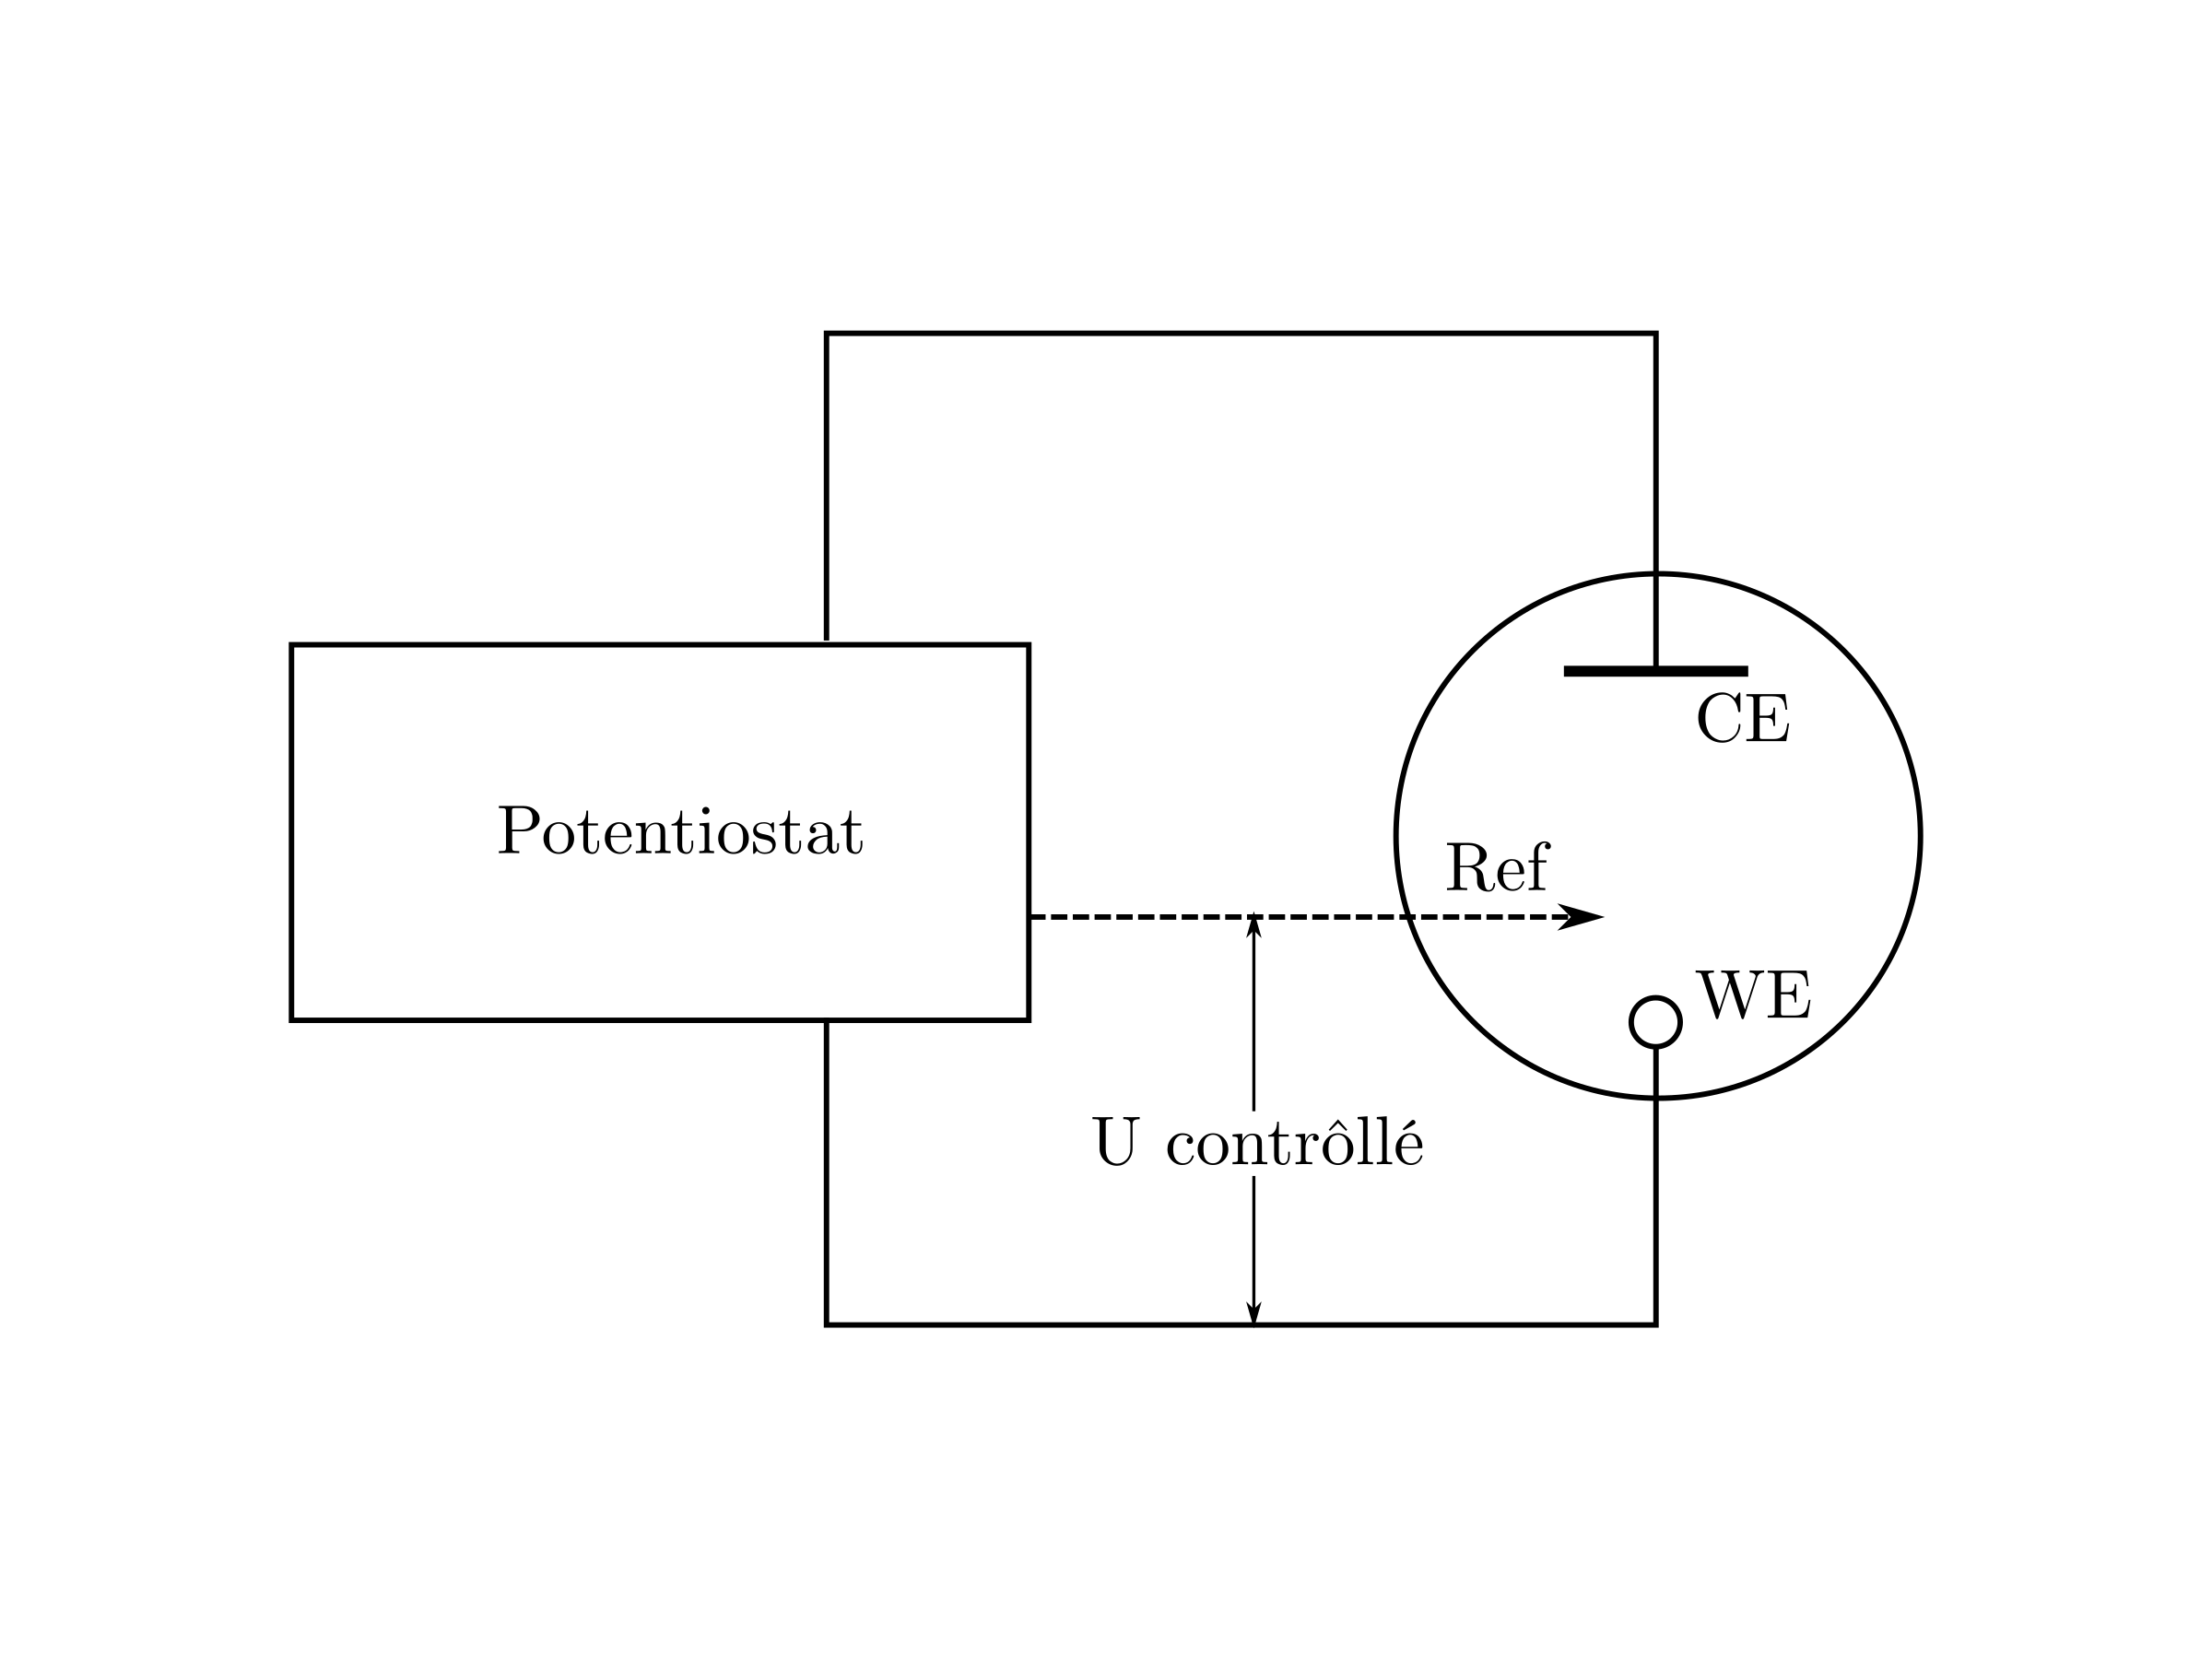
\includegraphics[width=0.65\textwidth]{Potentiostat_3E_Cell.png}
    %    \caption[Représentation schématique d'un potentiostat branché sur une cellule électrochimique à trois électrodes.]
    %    {Représentation schématique d'un potentiostat branché sur une cellule à trois électrodes \citep{Bard2001}.}
    %    \label{fig:ch2_potentiostat_3E_cell}
    %\end{figure}

    L'ensemble des mesures électrochimiques a été réalisé avec deux types de
    potentiostats: \emph{Solartron 1287} et \emph{Ametek PAR 4000}. 
    Les deux appareils peuvent fonctionner en mode flottant, ce qui était absolument nécessaire, le corps métallique de
    la cellule électrochimique développée étant mis à la terre pour des raisons de sécurité des personnes.

    \subsection{Mode flottant d'un potentiostat}
    
    Les micro-autoclaves instrumentés ainsi que la cellule électrochimique haute température, développée ici,
    peuvent être considérés comme des cellules électrochimiques à corps métallique,
    ce dernier permettant de chauffer la cellule à \SI{280}{\degreeCelsius} par le biais de colliers ou résistances
    chauffants. Par conséquent, les cellules de ce type doivent 
    être mises à la terre pour des raisons de sécurité.
    Afin de pouvoir réaliser des mesures électrochimiques correctes dans ces conditions difficiles, il est nécessaire
    que le potentiostat soit équipé d'un mode flottant, dans lequel le circuit de mesure et de contrôle
    utilisent une masse interne dont le potentiel peut "flotter" par rapport à la terre du réseau électrique.
    
    Ainsi en mode flottant, la borne contre-électrode du potentiostat peut être, si besoin est,    
    connectée directement sur le corps de la cellule  alors que
    l'électrode de travail est autorisée à "flotter" au potentiel contrôlé par le potentiostat 
    par rapport à la référence de potentiel.

    La figure \ref{fig:ch2_floating_mode} illustre les différences entre les modes de fonctionnement, flottant et non
    flottant, d'un potentiostat. 

    \begin{figure}[H]
        \centering
            
\includegraphics[width=0.60\textwidth]{Potentiostat_Floating_Mode.png}
        \caption[Représentation schématique des différences entre un système de contrôle/mesure non flottant 
        et un système de contrôle/mesure flottant.]
        {Représentation schématique des différences entre un système de contrôle/mesure non flottant et un système de
        contrôle/mesure flottant (d'après \citet{Barsoukov2005}).}
        \label{fig:ch2_floating_mode}
    \end{figure}

    

    \subsection{Suivis de potentiel électrochimique en circuit ouvert}\label{subsec:ch2_ECP}

    La mesure du potentiel électrochimique en circuit ouvert, également appelé couramment potentiel d'abandon, potentiel
    à l'équilibre ($U_{eq}$) ou OCV, a été réalisée via un potentiostat par rapport à une électrode de référence 
    comme illustré en figure \ref{fig:ch2_potentiostat_OCV}.
   
    Deux types d'électrode de référence ont été utilisés: fil de Pt et Ag/AgCl (KCl
    \SI{0.05}{\mole\per\liter}) \citep{King1989}. Le fil de Pt est une pseudo-référence et a été seulement utilisé dans les milieux désaérés
    des micro-autoclaves alors que l'électrode de référence Ag/AgCl \citep{King1989} a été principalement utilisée dans la cellule 
    électrochimique haute température (voir chapitre \ref{chap:design}).

    Il apparaît clairement que le potentiostat doit être équipé d'un mode flottant afin de mesurer correctement le
    potentiel électrochimique de l'électrode de travail (WE). Dans le cas où le potentiostat ne "flotte" pas, le
    potentiel mesuré est un potentiel mixte lié au couplage de l'électrode de travail (WE), virtuellement à la terre sur
    le potentiostat, avec le matériau
    métallique formant le corps de la cellule mis à la terre comme évoqué plus haut.

    \begin{figure}[H]
        \centering
            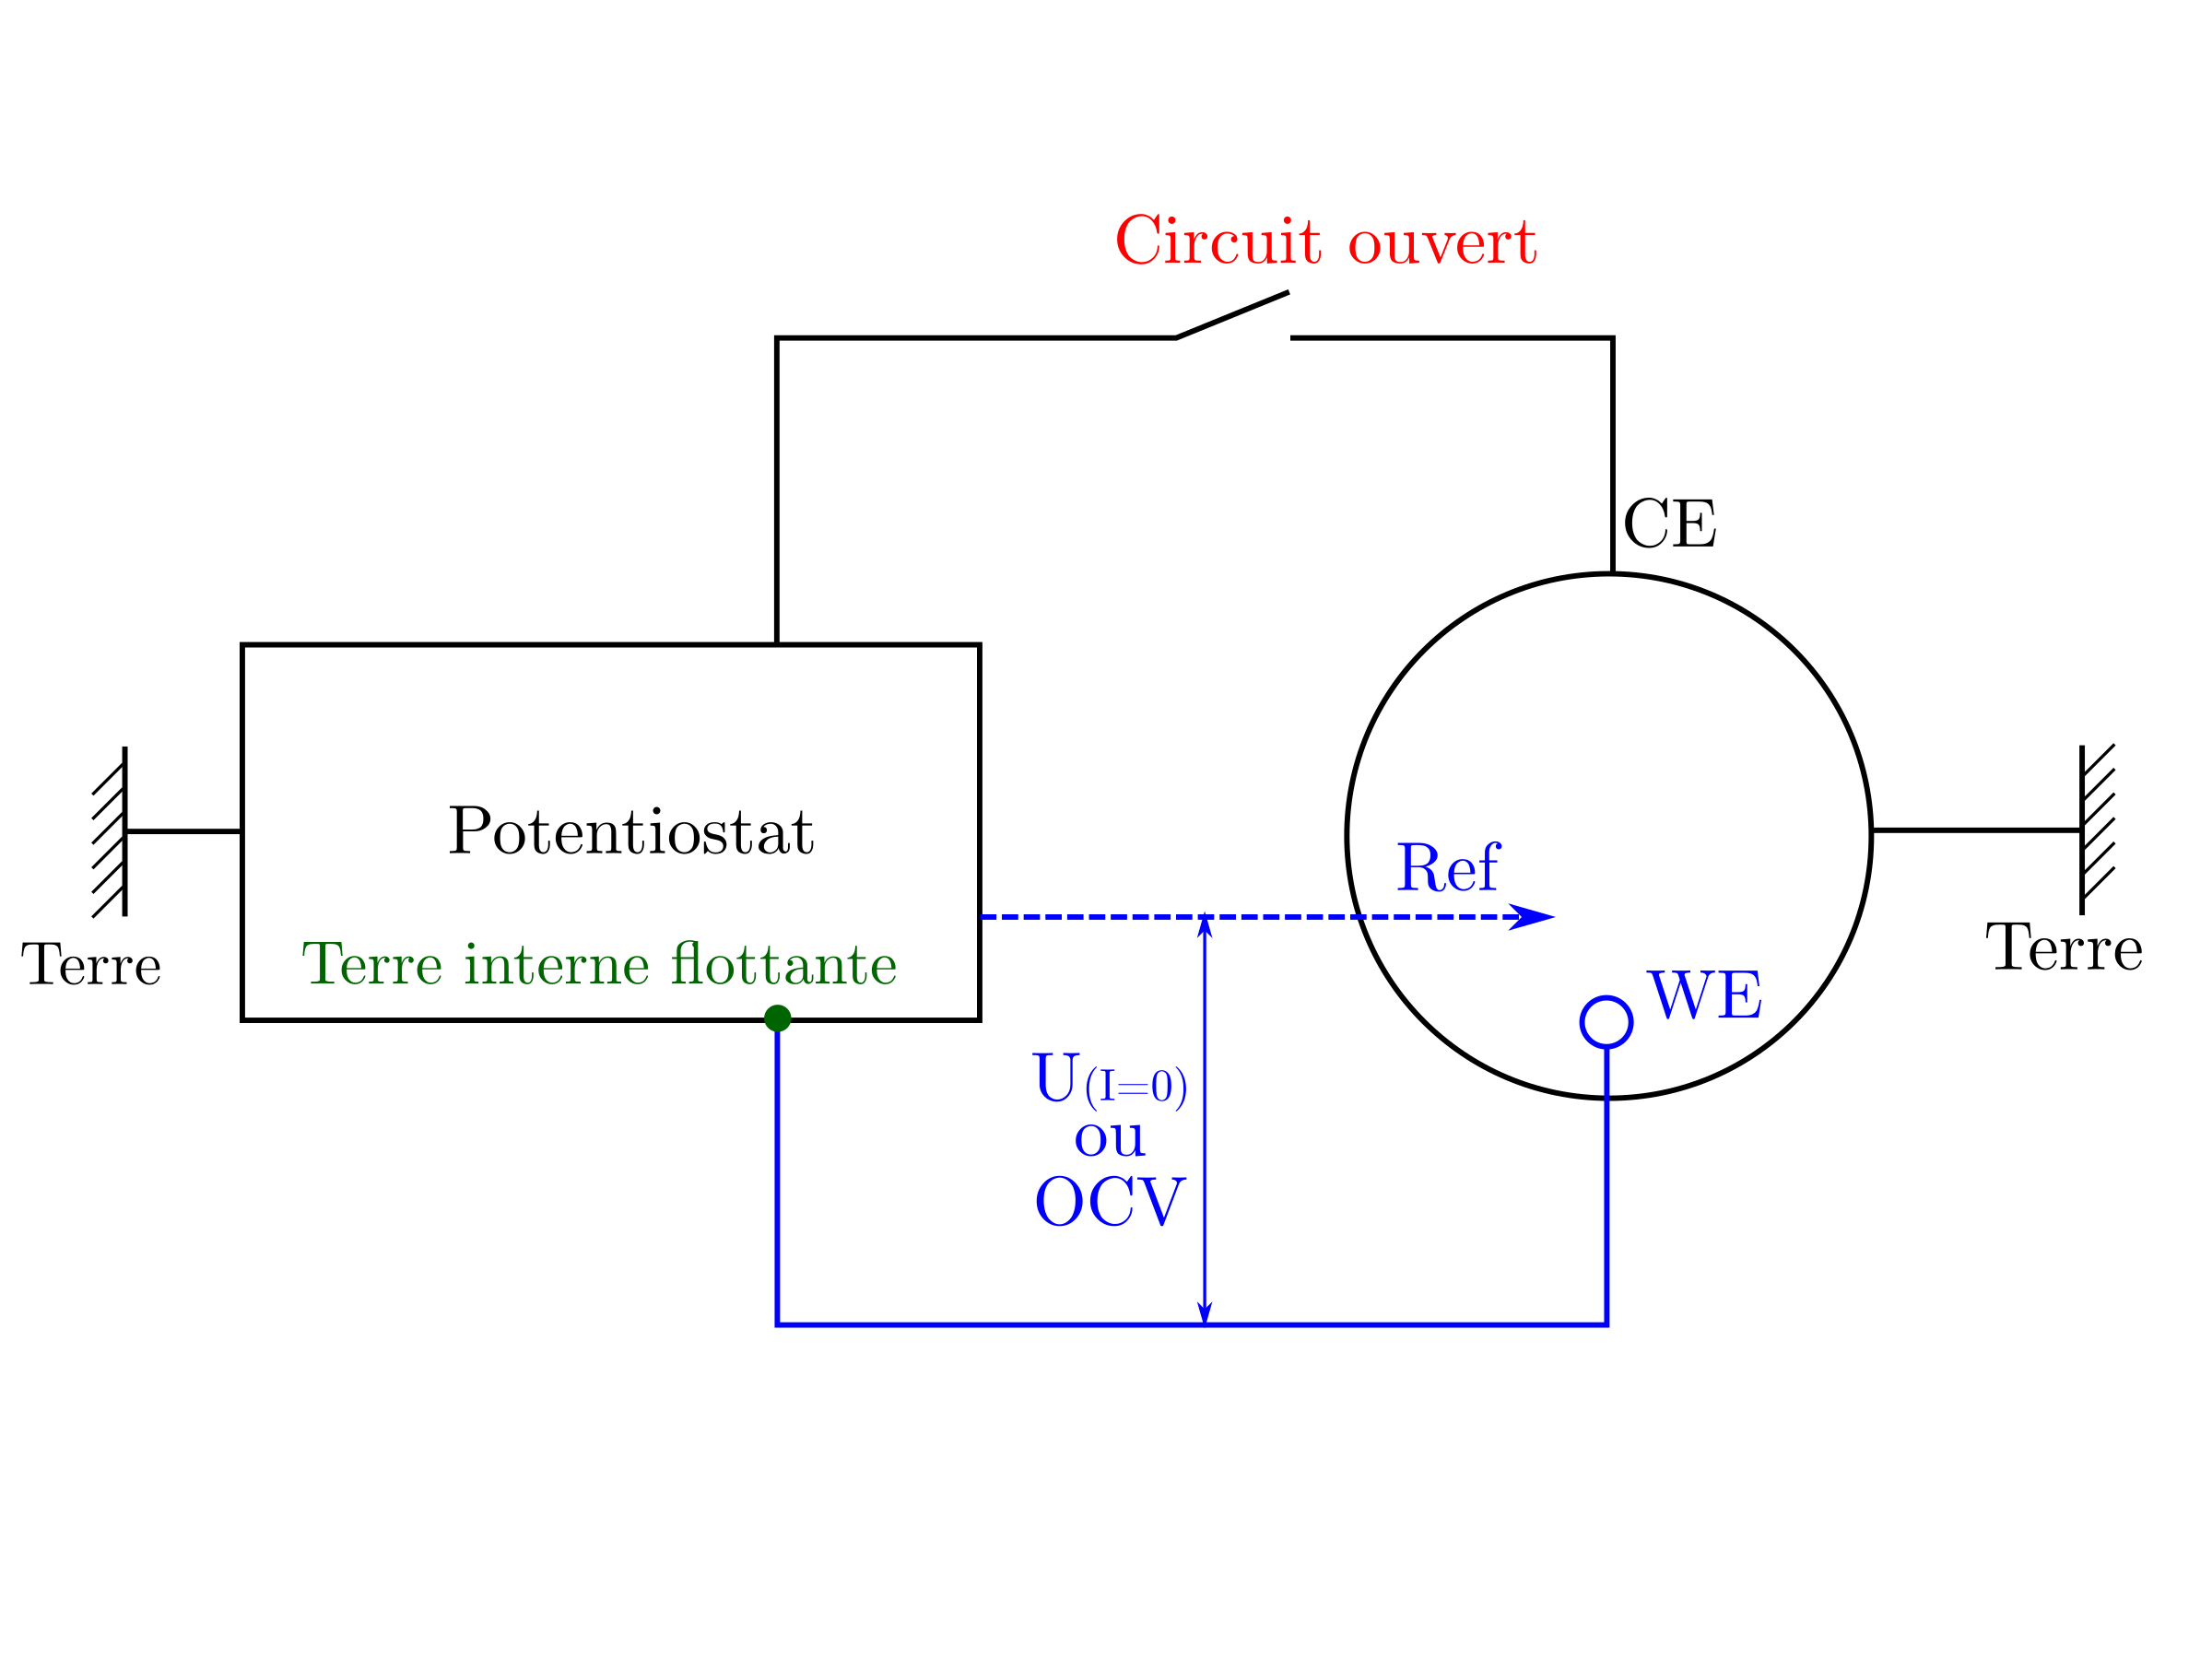
\includegraphics[width=0.65\textwidth]{Potentiostat_OCV.png}
        \caption{Représentation schématique d'un potentiostat flottant branché sur une cellule électrochimique à trois électrodes
        pour la mesure du potentiel électrochimique.}
        \label{fig:ch2_potentiostat_OCV}
    \end{figure}


    \subsection{Mesures des courbes de polarisation}\label{subsec:ch2_Tafel}

    La figure \ref{fig:ch2_potentiostat_Polarization} présente le branchement d'un potentiostat sur une cellule électrochimique
    avec un montage classique à trois électrodes. Les courbes de polarisations ont été enregistrées en imposant un balayage en
    potentiel de -10~mV (+10~mV) vs OCV à +200~mV (-200~mV)
    vs OCV pour une polarisation anodique (cathodique). La vitesse de balayage a été fixée à
    \SI{10}{\milli\volt\per\minute}. Cette vitesse de balayage faible permet de limiter la contribution de la décharge
    de la double couche électrochimique à chaque incrément de potentiel \citep{Talbot1998, Roberge1999, Kelly2003, Perez2004}.
    De plus, elle est préconisée par le standard ASTM G5.

    \begin{figure}[H]
        \centering
            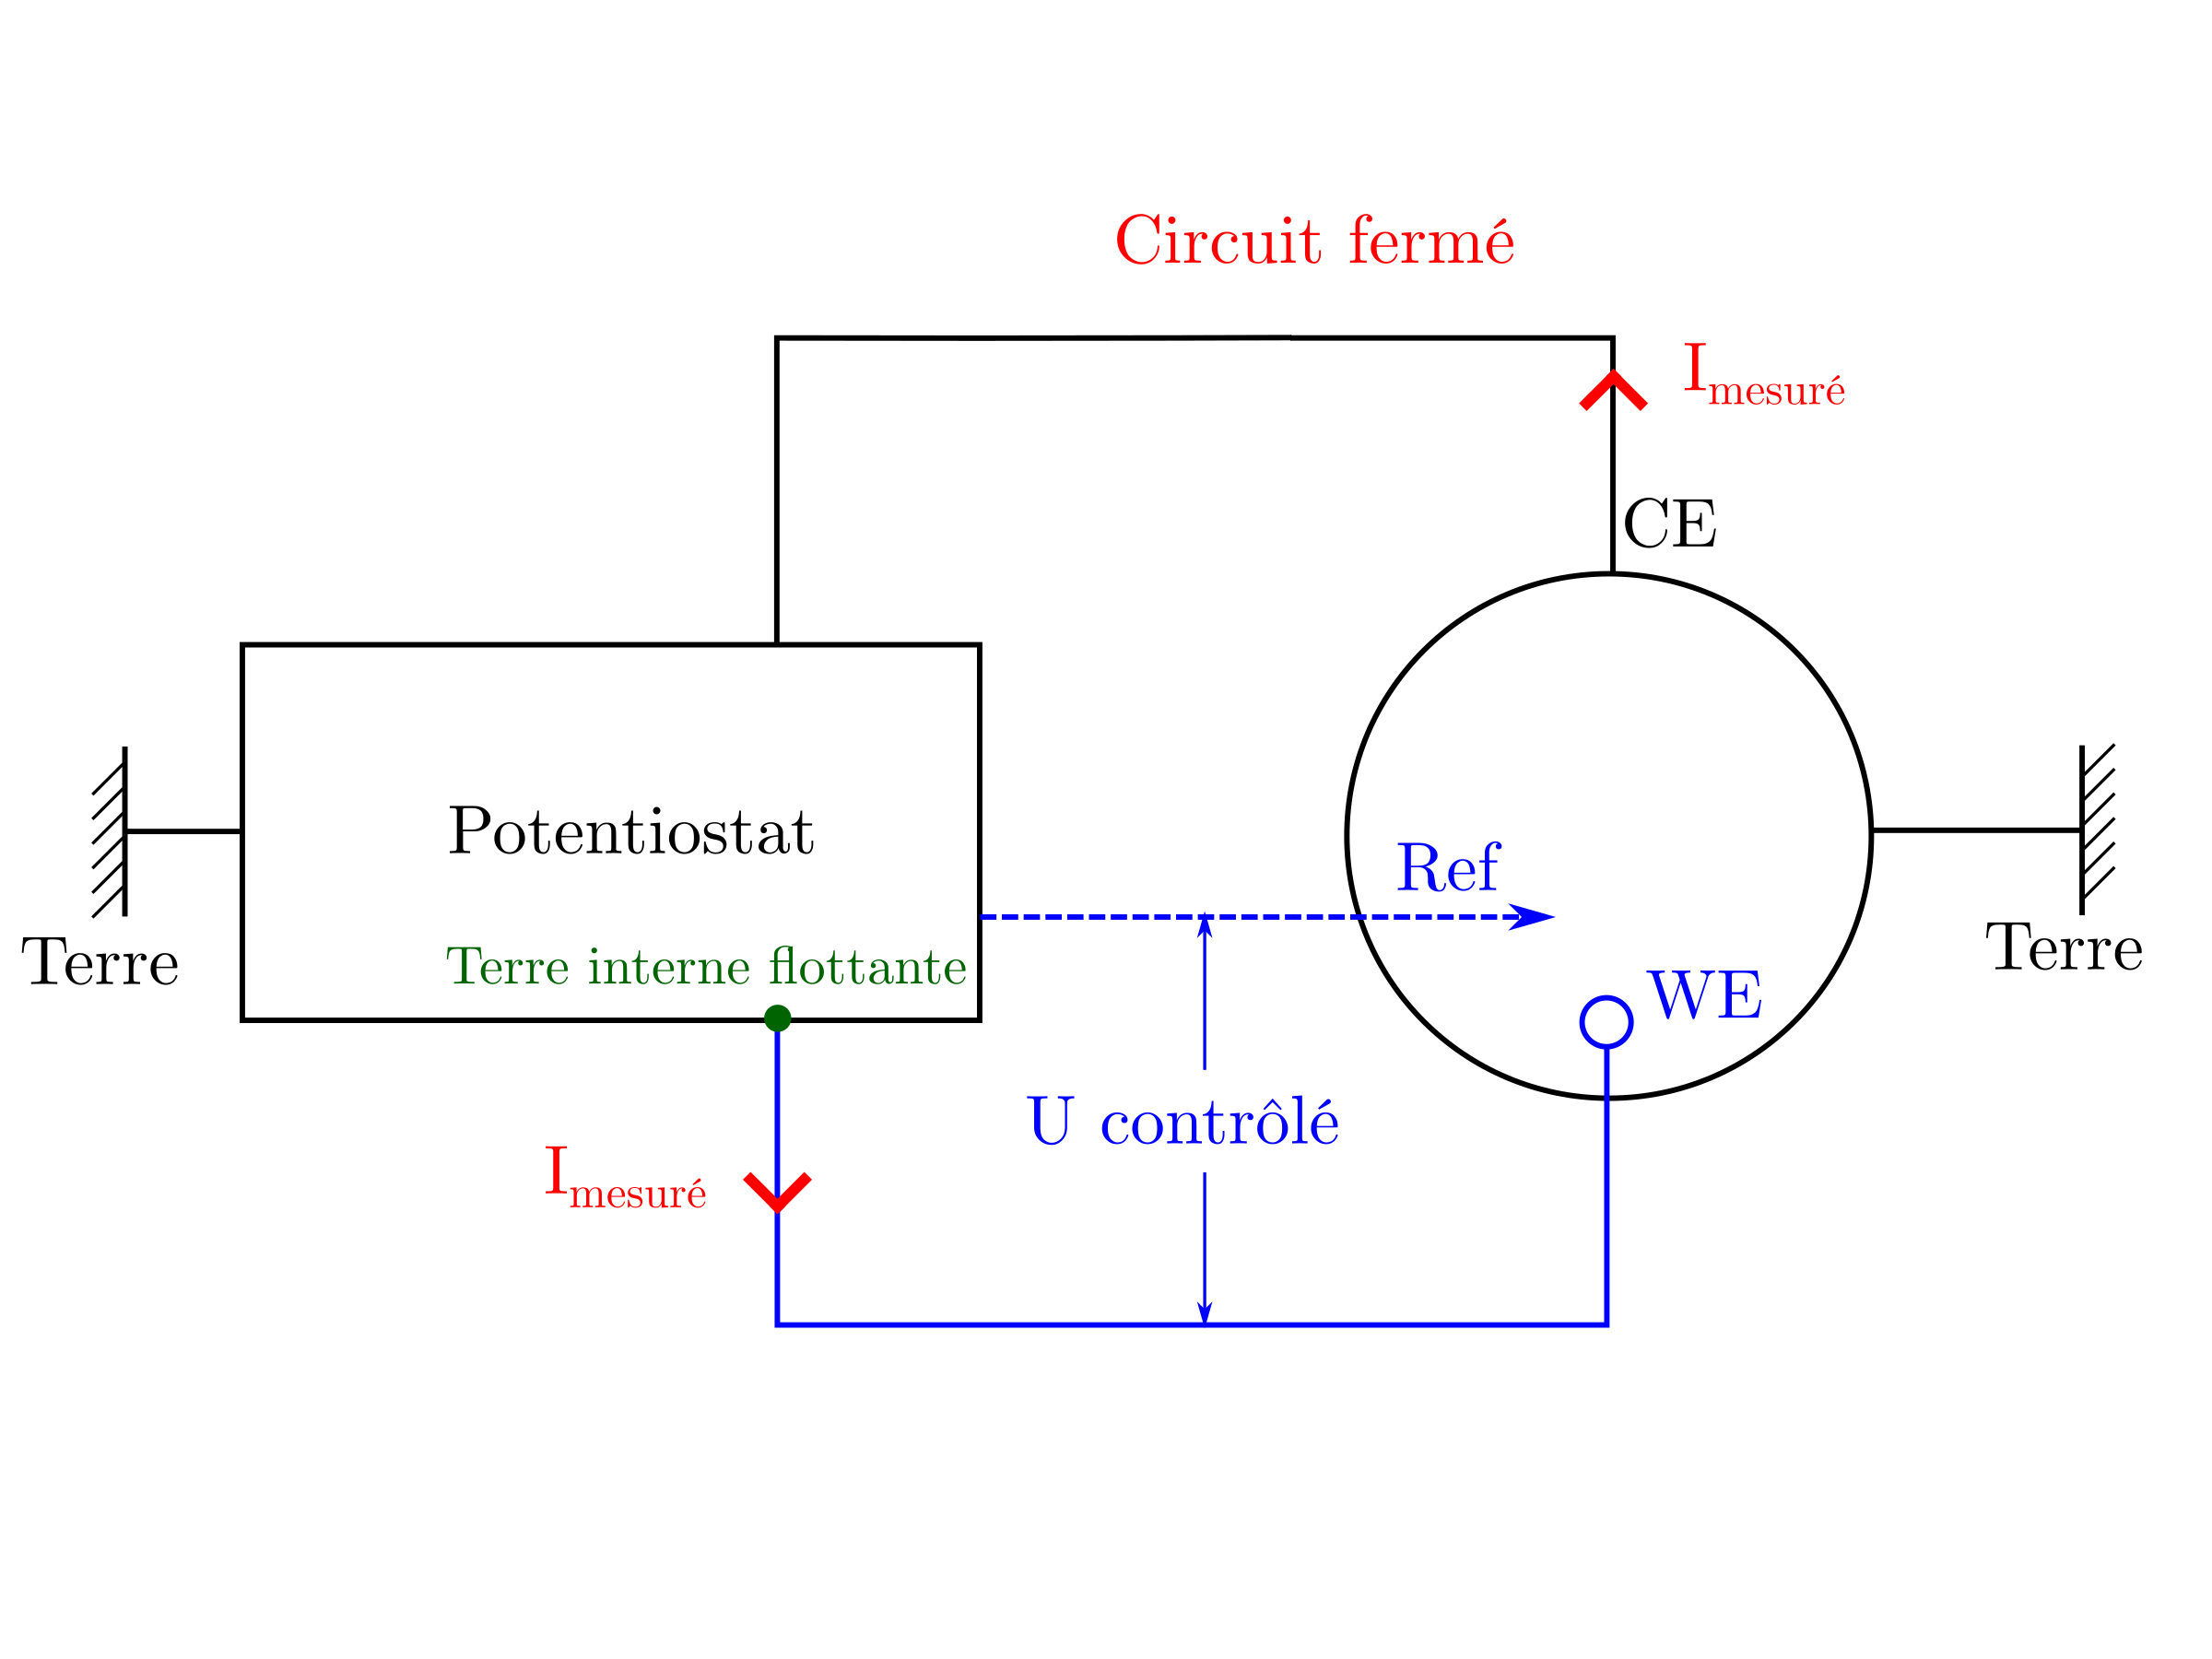
\includegraphics[width=0.65\textwidth]{Potentiostat_Polarization.png}
        \caption{Représentation schématique d'un potentiostat flottant branché sur une cellule électrochimique à trois
        électrodes pour la mesure des courbes de polarisation.}
        \label{fig:ch2_potentiostat_Polarization}
    \end{figure}


    La relation entre le courant électrochimique et le potentiel appliqué à l'électrode est décrite par l'équation
    de \emph{Butler-Volmer} pour une électrode métallique dont
    l'expression est donnée par l'équation \ref{eq:ch2_butler_volmer} dans l'hypothèse d'un processus limitant de transfert de charge. 
    $j$ représente la densité de courant, $j_0$ représente la densité de courant d'échange, U représente le potentiel
    électrochimique appliqué par rapport à une référence, $U_{eq}$ représente le potentiel électrochimique à
    l'équilibre mesuré par rapport à une référence, $\eta$ représente la surtension, $\alpha _a$ et $\alpha _c$ représentent les coefficients de
    transfert anodique et cathodique, z représente le nombre d'électrons échangés, R est la constante universelle
    des gaz parfaits et F est la constante de Faraday. 


    L'équation \ref{eq:ch2_butler_volmer} est valide si le système étudié 
    est un système lent c'est-à-dire que la limitation par le transport de matière n'apparaît que pour des surtensions
    importantes \citep{Bard2001, Diard1996}.
    Les couches d'oxydes formées sur les alliages Zy2 et Inc718 sont des couches passives dont la principale
    fonction est de ralentir la réaction d'oxydation et par conséquent la condition de validité de l'équation
    \ref{eq:ch2_butler_volmer} peut être considérée comme respectée.

    \begin{equation}
        \begin{split}
            j &= j_0 \left[ \exp\left(\frac{\alpha _az(U-U_{eq})}{RT/F}\right) 
            - \exp\left(-\frac{\alpha _cz(U-U_{eq})}{RT/F}\right) \right]\\
            j &= j_0 \left[ \exp\left(\frac{\alpha _az}{RT/F}\eta \right) 
            - \exp\left(-\frac{\alpha _cz}{RT/F}\eta \right) \right]\\
        \end{split}    
    \label{eq:ch2_butler_volmer}
    \end{equation}
    
    L'équation de \emph{Butler-Volmer} est la plus souvent utilisées en représentation de Tafel où l'on porte le
    logarithme de la valeur absolue de la densité de courant en fonction de la surtension $\eta$ comme illustré en
    figure \ref{fig:polarization_curve_n}. 
    
    \begin{figure}[H]
        \centering
        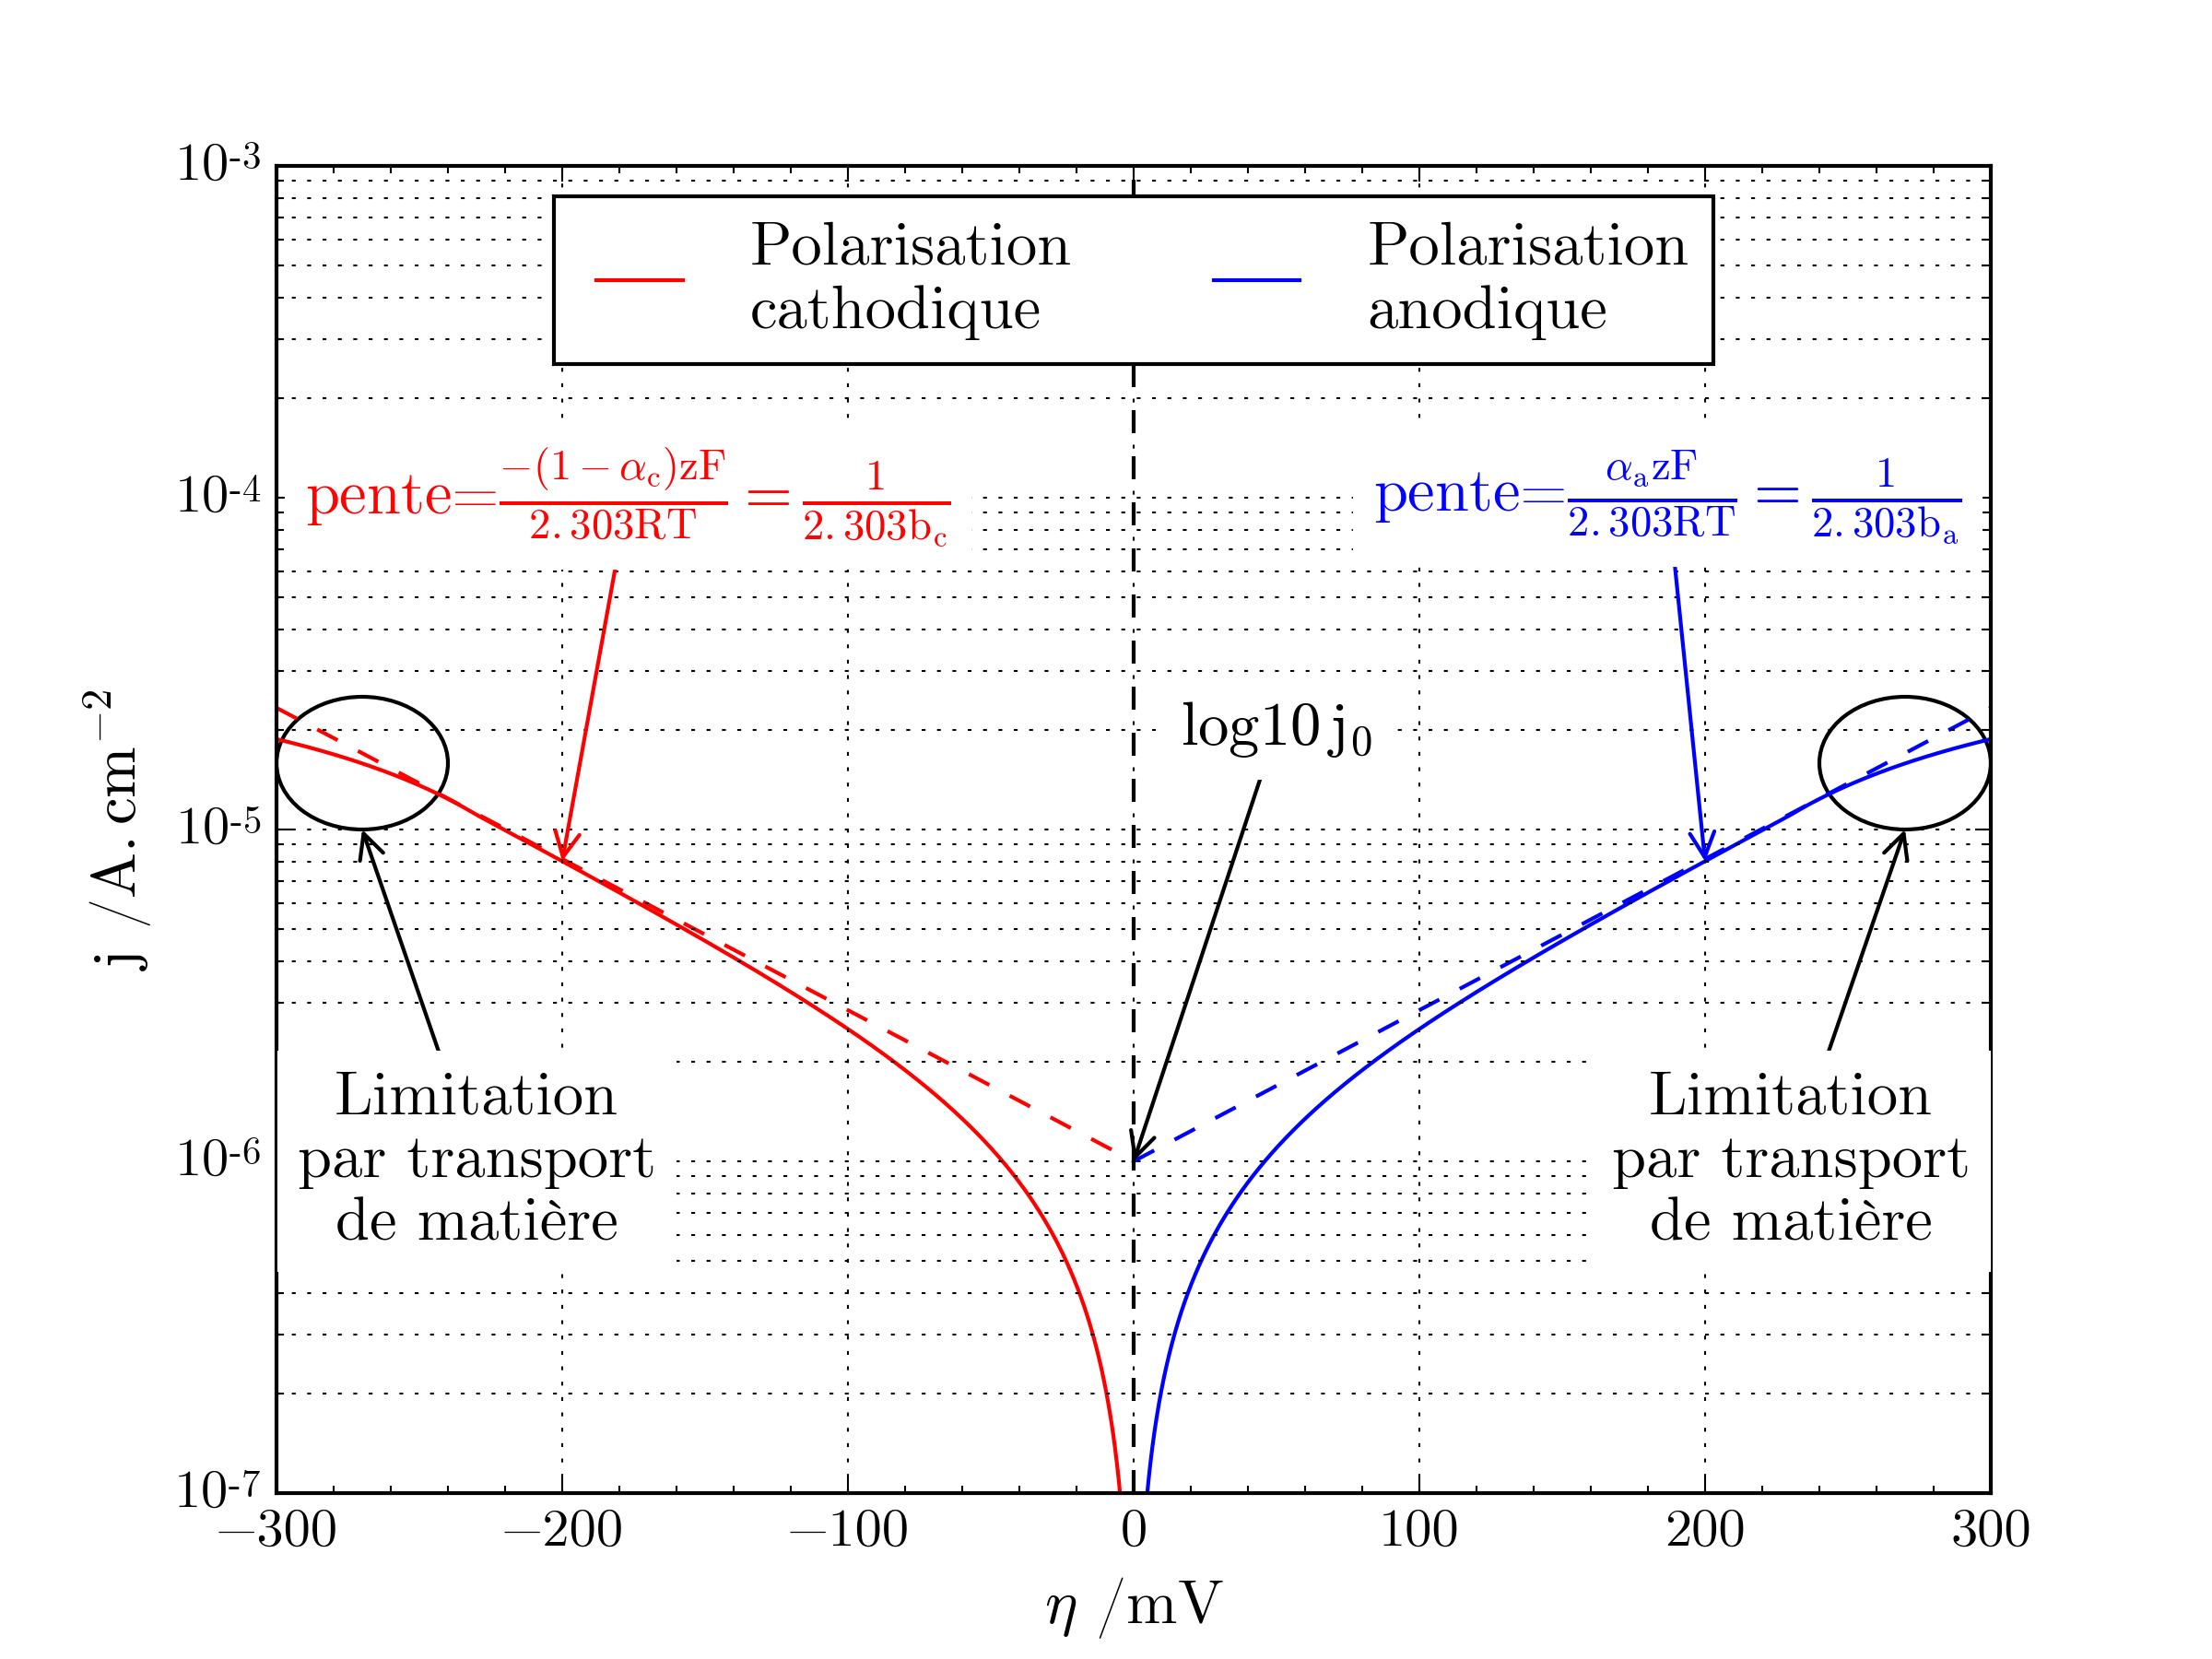
\includegraphics[width=0.65\textwidth]{Polarization_Curve-n.png}
        \caption{Représentation de Tafel des branches anodiques et cathodiques du courant en fonction de la surtension $\eta$.}
        \label{fig:polarization_curve_n}
    \end{figure}
    
    Dans ces conditions
    aux potentiels plus anodiques que le potentiel d'équilibre (ce qu'on appelle la branche anodique) comme aux
    potentiels plus cathodiques (ce qu'on appelle la branche cathodique) on obtient deux droites de pentes $b_a$ et $b_c$
    également appelées pentes de Tafel. Les pentes de Tafel sont liées aux coefficients de transfert par
    l'équation \ref{eq:ch2_link_b_alpha} avec RT/F (=kT/e) valant \SI{47.7}{\milli\volt} et \SI{25.7}{\milli\volt} 
    à \SI{280}{\degreeCelsius} et \SI{25}{\degreeCelsius}, respectivement.

    \begin{equation}
         b = \frac{kT}{e \alpha z} = \frac{RT}{F \alpha z}   
         \label{eq:ch2_link_b_alpha}
    \end{equation}

    \noindent En introduisant les pentes de Tafel, l'équation \ref{eq:ch2_butler_volmer}
    peut être exprimée sous la forme de l'équation \ref{eq:ch2_butler_volmer_ba_bc}:
    
    \begin{equation}
         j = j_0 \left[ \exp\left( \frac{\eta}{b_a}\right) - \exp\left( -\frac{\eta}{b_c}\right)  \right] 
    \label{eq:ch2_butler_volmer_ba_bc}
    \end{equation}

    Comme mentionné précédemment, la zone linéaire dans la représentation de Tafel n'apparaît seulement que si le système est lent.
    Dans la plupart des cas, la zone de linéarité est observée lorsque la surtension en unité de kT/e ($\left|
    \frac{\eta}{kT/e} \right|$) est comprise entre 1 et 5.
    A \SI{280}{\degreeCelsius}, cela correspond à une surtension, $\vert \eta \vert$, comprise entre environ \SI{
    48}{\milli\volt} et environ \SI{240}{\milli\volt}. 

    Les mesures brutes des courbes de polarisation sont corrigées de la résistance d'électrolyte et normalisées à la
    surface géométrie exposée dans l'électrolyte.
    La densité de courant d'échange, $j_0$, et la pente de Tafel, b, seront déterminés par régression linéaire avec la
    méthode des moindres carrés.
    Le coefficient de transfert de charge, $\alpha$, en sera déduit avec l'équation \ref{eq:ch2_link_b_alpha}. Il faut tout
    de même mentionner que l'obtention par régression linéaire de ces paramètres reste une approximation car les courbes réelles
    sont toujours plus bruitées et les limites de la zone de linéarité ne sont pas toujours aisées à déterminer.  

    Les courbes de polarisation permettent également de déterminer la densité de courant de couplage entre deux
    matériaux
    tels que Zy2 et Inc718.
    En effet, l'intersection de la branche anodique, du matériau en situation d'oxydation, et de la branche cathodique, du
    matériau en situation de réduction, définit la densité de courant de couplage. Cette dernière peut être également
    mesurée directement. 
    
    
    \subsection{Mesures directes des courants de couplage}\label{subsec:ch2_ZRA}

    Ces mesures directes du courant de couplage ont été obtenues avec dispositif de résistance nulle plus communément appelé ZRA
    \citep{Gabrielli2015}. D'un
    point vue électronique, c'est un montage suiveur de courant \citep{Bard2001}. La plupart des potentiostats modernes
    sont équipés d'un mode ZRA permettant ainsi de mesurer un courant de couplage entre deux matériaux 
    considérés comme deux électrodes de travail (WE1 et WE2) dont une électrode devient l'anode et l'autre la cathode.
    De plus, il est possible de mesurer le potentiel mixte par rapport à une référence de potentiel.

    La figure \ref{fig:ch2_potentiostat_ZRA} présente le branchement d'un potentiostat sur une cellule électrochimique
    avec deux électrodes de travail. Ces dernières sont branchées sur la masse interne flottante avec un ZRA disposé entre
    les deux points de branchement. Il faut noter que dans ce cas de figure, la contre-électrode n'est pas utilisée. 
    Ce type de branchement est également utilisé pour mesurer le bruit électrochimique.

    \begin{figure}[!htb]
        \centering
            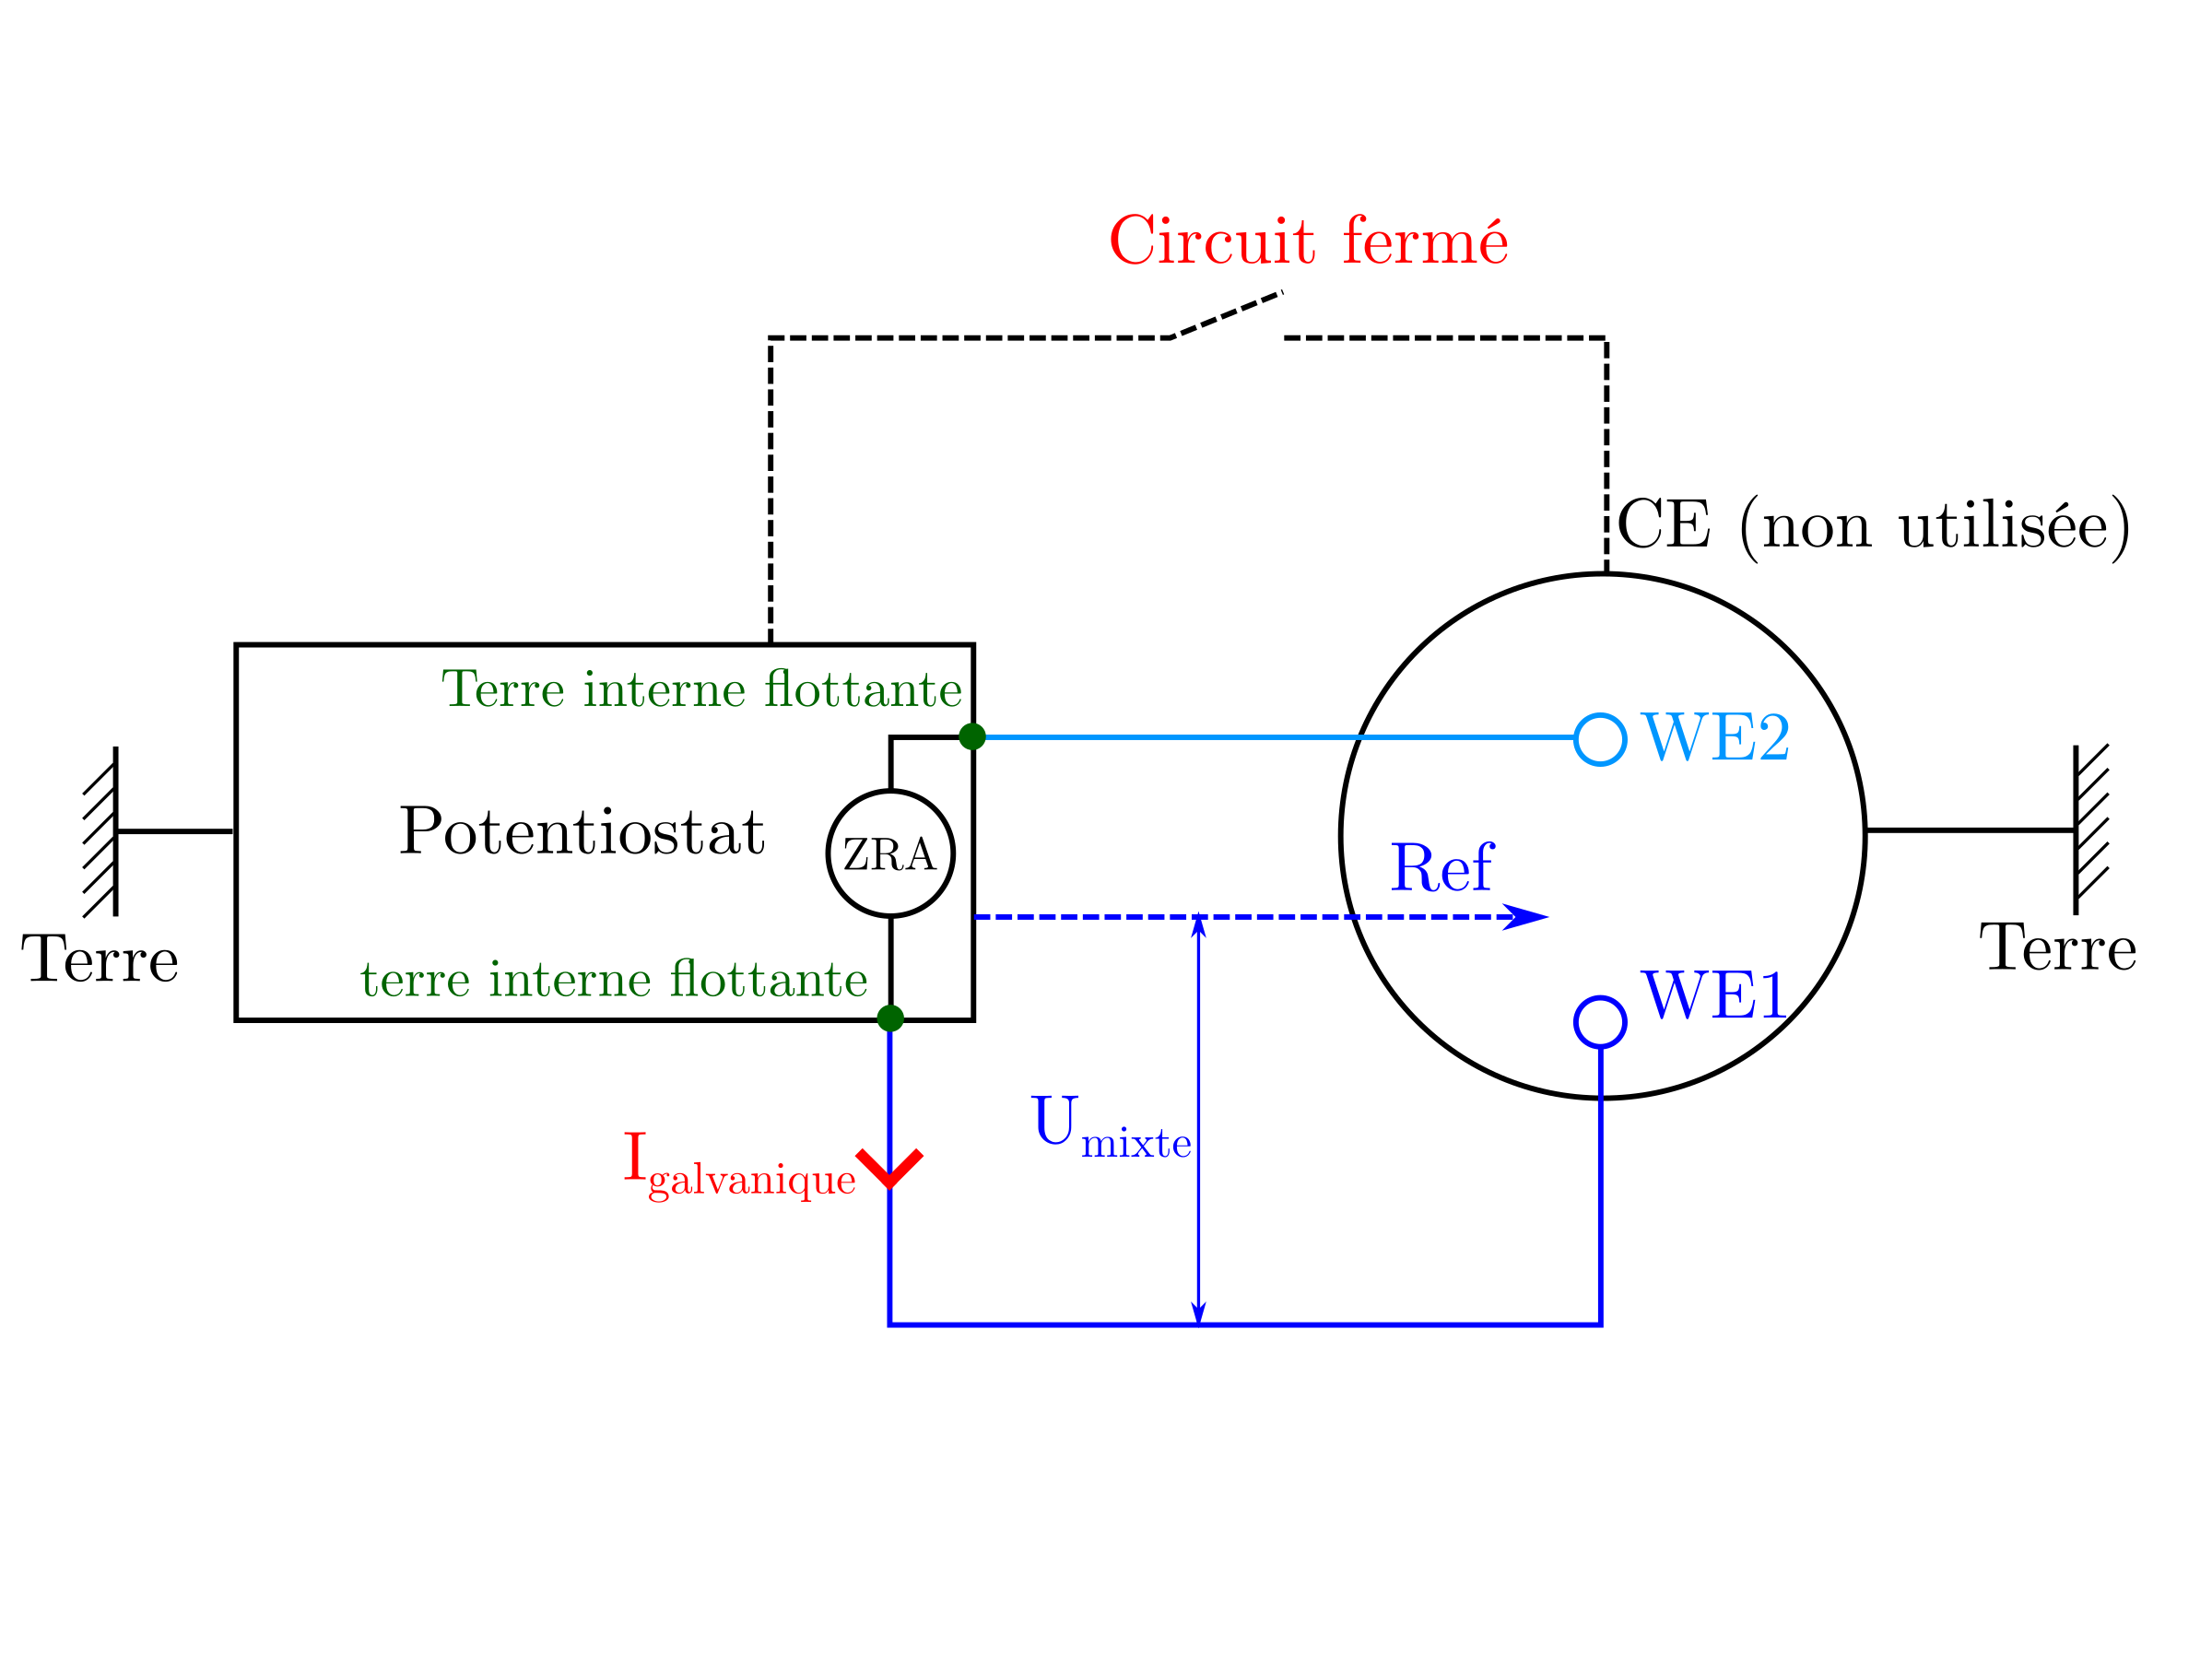
\includegraphics[width=0.65\textwidth]{Potentiostat_ZRA.png}
        \caption{Représentation schématique d'un potentiostat flottant branché sur une cellule électrochimique avec deux
        électrodes de travail pour la mesure du potentiel mixte et du courant de couplage.}
        \label{fig:ch2_potentiostat_ZRA}
    \end{figure}

    L'équation \ref{eq:ch2_jgalvanic} montre que la densité de courant de couplage, $j_{gal}$, 
    a été obtenue en normalisant le courant de couplage, $I_{gal}$, à la surface géométrique de
    l'anode, $S_a$. 
        
    \begin{equation}
        j_{gal} = \frac{I_{gal}}{S_{a}}
    \label{eq:ch2_jgalvanic}
    \end{equation}

    Cette densité de courant est une mesure directe pour un certain rapport de surface géométrique exposée dans
    l'électrolyte, $r_s$, entre la cathode ($S_c$) et l'anode ($S_a$). 
    La densité de courant ainsi calculée ne peut pas être comparée
    directement à la valeur obtenue sur les courbes de polarisation.
    Comme déjà mentionné précédemment (\S\ref{subsec:ch2_Tafel}), la densité de courant de couplage, obtenue à
    l'intersection des branches anodiques et cathodiques, correspond à un rapport de surface de 1. Par conséquent, il
    est nécessaire de corriger la mesure directe afin de se replacer dans la situation d'un rapport de surface de 1. 
    La correction à appliquer consiste à diviser la mesure directe, $j_{gal}$, par le rapport de surface $r_s$ comme
    illustré par l'équation \ref{eq:ch2_jgalvanic_correction}.

    \begin{equation}
        j_{gal}^{\prime} = \frac{j_{gal}}{r_s} \text{ avec } r_s = \frac{S_c}{S_a}
    \label{eq:ch2_jgalvanic_correction}
    \end{equation}


    
    

    
    


%%%%%%%%%%%%%%%%%%%%%%%%%%%%%%%%%%%%%%%%%%%%%%%%%%%%%
\section{Remarques de conclusion}

    Les micro-autoclaves statiques instrumentés permettent de tester les alliages Zy2 et Inc718 dans un milieu REB
    simulé 
    monophasique (sans ébullition), mais le contrôle fin de l'oxygène dissous n'est pas possible, ce qui impose de
    travailler avec des électrolytes désaérés. 

    Les méthodes électrochimiques permettent d'obtenir des paramètres liés au comportement électrochimique des alliages
    Zy2 et Inc718, et sont parfaitement adaptées pour l'étude du mécanisme de couplage galvanique, proposé
    entre autres par
    \citet{Lysell2004} (ch.\ref{chap:ch1_bib}, \S\ref{subsec:galvanic_coupling}), dans les conditions expérimentales des
    micro-autoclaves.

    Néanmoins, l'impact de l'illumination UV ne peut être testé en micro-autoclave. Afin de s'affranchir de cette
    limitation, une nouvelle cellule électrochimique haute température a été développée permettant d'illuminer les échantillons. 
    En plus de permettre
    d'appliquer les méthodes électrochimiques, évoquées dans ce chapitre, cette nouvelle cellule offrira la possibilité de
    réaliser des tests ou caractérisations photoélectrochimiques en lumière poly ou monochromatique.
    
    Enfin, l'utilisation d'une boucle de contrôle de la chimie reliée à la cellule lèvera
    la limitation sur le contrôle fin de l'oxygène dissous dans le milieu REB simulé.
    La conception et développement et la validation de ce dispositif expérimental original font l'objet du prochain
    chapitre.
    \singlespacing
\printbibliography[heading=subbibintoc]
    \onehalfspacing
\end{refsection}
